% This is a LaTeX thesis template for Adam Mickiewicz University.
% to be used with Rmarkdown
% This template was produced by Jakub Nowosad
% Version: 16 February 2020

% Inspired by:
% This is a LaTeX thesis template for Monash University.
% to be used with Rmarkdown
% This template was produced by Rob Hyndman
% Version: 6 September 2016

\documentclass{amuthesis}
% \usepackage[polish]{babel}
\usepackage{polski}
\renewcommand{\figurename}{Rycina} % Redefine default figure caption %
\renewcommand{\tablename}{Tabela} % Redefine default table caption %
%%%%%%%%%%%%%%%%%%%%%%%%%%%%%%%%%%%%%%%%%%%%%%%%%%%%%%%%%%%%%%%
% Add any LaTeX packages and other preamble here if required
%%%%%%%%%%%%%%%%%%%%%%%%%%%%%%%%%%%%%%%%%%%%%%%%%%%%%%%%%%%%%%%
\usepackage{booktabs,tabularx} % Allows kableExtra to work %
\usepackage{indentfirst} % Adds indent in the first paragraph %
\usepackage{bookmark} % Adds indent in the first paragraph %

\author{Błażej Kościański}
\title{Porównanie miar niepodobieństwa struktury przestrzennej w
kontekście określania zmian kategorii pokrycia terenu}
\def\titleeng{Comparison of spatial structure dissimilarity measures in
the context of determining land cover changes}
\def\degreetitle{Praca magisterska}
\def\major{Geoinformacja}
\def\albumid{444861}
\def\thesisyear{2024}

% Add subject and keywords below
\hypersetup{
     %pdfsubject={The Subject},
     %pdfkeywords={Some Keywords},
     pdfauthor={Błażej Kościański},
     pdftitle={Porównanie miar niepodobieństwa struktury przestrzennej w
kontekście określania zmian kategorii pokrycia terenu},
     pdfproducer={quarto with LaTeX}
}

\bibliography{thesis.bibpackages.bib}

\begin{document}

\pagenumbering{arabic}

\titlepage

\bookmarksetup{startatroot}

\hypertarget{streszczenie}{%
\chapter*{Streszczenie}\label{streszczenie}}
\addcontentsline{toc}{chapter}{Streszczenie}

\markboth{Streszczenie}{Streszczenie}

\textbf{Abstrakt}

Analiza zmian w pokryciu terenu w różnych okresach czasowych lub między
różnymi zestawami danych obrazowych stanowi istotne zagadnienie w
badaniach geoprzestrzennych. Istnieje szereg technik służących do
analizy różnic w danych rastrowych, w tym metody oparte na analizie
struktur przestrzennych. W tych metodach, stopień zróżnicowania dwóch
obszarów może być oszacowany za pomocą miar odległości, podobieństwa,
niepodobieństwa i innych wskaźników. Współcześnie jednak nie określono,
która z tych miar najlepiej odzwierciedla ludzkie postrzeganie różnic w
pokryciu terenu. Celem tej pracy było porównanie metod określania zmian
struktury przestrzennej kategorii pokrycia terenu z postrzeganiem zmian
przestrzennych przez ludzi. W tym celu przeprowadzona została ankieta w
której zadaniem respondentów była ocena podobieństwa między parami
rastrów. Zbiory danych rastrowych zostały przygotowane poprzez symulację
parametrów kompozycji i konfiguracji przestrzennej. W analizie
uwzględniono 20 miar niepodobieństwa oraz dwie miary z dziedziny teorii
informacji: entropia brzegowa i względna informacja wzajemna. W efekcie
przeprowadzonych badań udało się opisać relacje między sposobem
postrzegania przez ludzi różnic w pokryciu terenu a wynikami miar
niepodobieństwa oraz wartościami miar opisujących kompozycję i
konfigurację przestrzenną par rastrów.

Słowa kluczowe: zmiany pokrycia terenu, struktura przestrzenna, miary
odległości, miary niepodobieństwa, ekologia krajobrazu

\newpage

\textbf{Abstract}

The analysis of changes in land cover over different time periods or
between different image datasets is an important issue in geospatial
research. There are a number of techniques for analysing differences in
raster data, including pattern-based change assessment methods. In these
methods, the difference between two areas can be estimated using
measures of distance, similarity, dissimilarity and other indicators.
However, at present, it has not been determined which of these measures
best reflects human perception of differences in land cover. The aim of
this work was to compare methods for determining changes in the spatial
structure of land cover categories with human perceptions of spatial
change. For this purpose, a survey was conducted in which respondents
were asked to assess the similarity between pairs of rasters. The raster
datasets were prepared by simulating composition and spatial
configuration parameters. The analysis included 20 measures of
dissimilarity and two information theory measures: marginal entropy and
relative mutual information. As a result of the study, it was possible
to describe the relationships between people's perceptions of
differences in land cover and the results of dissimilarity measures and
the values of measures describing the spatial composition and
configuration of raster pairs.

Keywords: land cover changes, spatial pattern, distance measures,
dissimilarity measures, landscape ecology

\newpage

\setstretch{1.2}\sf\tighttoc\doublespacing

\bookmarksetup{startatroot}

\hypertarget{sec-wprowadzenie}{%
\chapter{Wprowadzenie}\label{sec-wprowadzenie}}

Informacje geograficzne są wynikiem selekcji i przetwarzania danych
związanych z otaczającą nas przestrzenią geograficzną. Pozwalają na
bardziej zrozumiałe i efektywne analizowanie, modelowanie oraz
interpretowanie złożonych zjawisk i procesów zachodzących w naszym
otoczeniu. Informacje geograficzne i ich aspekty nie stanowią
niepodważalnych faktów, lecz często powstają w wyniku działań jednostek,
jak i wspólnych wysiłków grup ekspertów, którzy zajmują się wyborem,
analizą i klasyfikacją danych geograficznych \autocite{WhatIsLandCover}.
W procesie tworzenia informacji geograficznych istnieje zatem pewien
stopień subiektywności, który może wpłynąć na ostateczną postać tych
informacji, ich interpretację, jak i na ich użyteczność w kontekście
innych zastosowań. Przykładem informacji geograficznej, której
ostateczna postać zależna jest od założeń przyjętych w trakcie tworzenia
danych przestrzennych, jest pokrycie terenu.

Przyjmuje się, że termin pokrycie terenu obejmuje zbiór wszelkich
elementów obecnych na powierzchni Ziemi \autocite{Fisher2005}. W
elementy pokrycia terenu włączają się obiekty związane z działalnością
człowieka, skutkami sił przyrody oraz wszelkie inne istniejące obiekty,
które mogą znaleźć się w przestrzeni geograficznej
\autocite{zwolinski2018}. Tworzenie dokładnych i wiarygodnych danych
dotyczących pokrycia terenu jest niezbędne w kontekście wielu
zastosowań, takich jak planowanie przestrzenne
\autocite{bibby1999monitoring}, ochrona środowiska
\autocite{natura2000_land_cover}, czy analiza zmian klimatycznych
\autocite{dravskovic2020climate}. Ostateczna forma tych danych jest
jednak w dużej mierze determinowana przez wybory i założenia dokonywane
w procesie ich tworzenia. W tym kontekście, analiza pokrycia terenu
staje się istotnym polem badań, które skupia się na zarówno na
technicznych aspektach zbierania danych, jak i na ich semantycznej
interpretacji.

Dane oraz wynikowe mapy pokrycia terenu są rezultatem złożonego procesu
przetwarzania i analizy informacji przestrzennych najczęściej w postaci
obrazów satelitarnych
\autocite{ChangeDetectionTechniques,Jasiewicz_GeoPAT}. Na początku tego
procesu, satelity wyposażone w sensory rejestrują obrazy Ziemi z różnych
zakresów widmowych. Dane pochodzące z teledetekcji często mają postać
danych rastrowych, gdzie informacje przestrzenne są zapisane w formie
regularnej siatki komórek lub punktów \autocite{glazewski2006modele}. W
modelu danych rastrowych każda z tych komórek lub punktów przechowuje
jedną wartość, która stanowi reprezentację jakiejś charakterystyki
danego fragmentu powierzchni Ziemi. Obrazy uzyskane w procesie
teledetekcji mogą być interpretowane manualnie przez grupy specjalistów.
Pozwala to na uzyskanie map pokrycia terenu o wysokiej dokładności,
kosztem długiego procesu ich tworzenia \autocite{CUNNINGHAM2006217}.
Dużo mniej czasochłonną metodą jest przetwarzanie przy użyciu
algorytmów. Umożliwiają one względnie szybką, półautomatyczną
identyfikację i klasyfikację różnych typów powierzchni kosztem mniejszej
dokładności mapy wynikowej \autocite{CUNNINGHAM2006217}. Ostatecznie,
dane przekształcone w mapy pokrycia terenu mogą posłużyć do analiz zmian
pokrycia terenu \autocite{Feranec2007,Sleeter2013,Mierzwiak_Całka_2019}.

Celem analiz zmian pokrycia terenu jest przede wszystkim monitorowanie i
pogłębienie aktualnej wiedzy na temat ewolucji otaczającego nas
krajobrazu \autocite{ChangeDetectionTechniques}. Jest to istotne w
kontekście ochrony przyrody \autocite{lulcc_natura2000}, planowania
przestrzennego \autocite{urbanplanning}, oceny wpływu inwestycji i
infrastruktury na środowisko \autocite{infrastructure_environment}, a
także w badaniach dotyczących zmian klimatycznych
\autocite{lulcc_climate_change}, bioróżnorodności
\autocite{lulcc_biodiversity} oraz innych procesów ekologicznych
\autocite{ChangeDetectionTechniques}. Dzięki analizie zmian pokrycia
terenu można identyfikować obszary zagrożone degradacją, monitorować
skutki urbanizacji, deforestacji czy erozji, co umożliwia podejmowanie
odpowiednich działań w celu zrównoważonego zarządzania środowiskiem i
zachowaniem jego integralności.

W badaniach nad zmianami pokrycia terenu wykorzystuje się różnorodne
metody analityczne. Niemniej jednak, wiele z tych technik koncentruje
się na analizie zmian na poziomie indywidualnych komórek w siatce rastra
\autocite{ChangeDetectionTechniques}. Choć podejście to może dostarczać
użytecznych informacji dotyczących trendów zmian pokrycia terenu na
niewielkich obszarach, charakteryzuje się ono istotnymi ograniczeniami w
kontekście interpretacji wyników. Szczególnie w przypadku badań
obejmujących rozległe terytoria, takie jak kraje czy nawet kontynenty,
bardziej efektywne staje się zastosowanie metod opartych na analizie
struktur przestrzennych \autocite{Netzel2015}. Głównym założeniem tych
metod jest przekształcenie danych z postaci pojedynczych wartości
komórek rastra w sygnatury przestrzenne, a następnie porównanie ich ze
sobą za pomocą miar odległości i niepodobieństwa.

Sygnatury przestrzenne stanowią statystyczny opis struktur
przestrzennych kategorii pokrycia terenu na mniejszych, wydzielonych
obszarach w obrębie całego zbioru danych. W celu porównania ze sobą
dwóch sygnatur przestrzennych, wykorzystywane są miary niepodobieństwa.
Umożliwiają one określenie w jakim stopniu dwa analizowane obszary się
od siebie różnią pod względem kompozycji oraz konfiguracji
przestrzennej. Opracowane zostało wiele różnych miar niepodobieństwa,
takich jak odległość euklidesowa, odległość Canberra, metryka Wave
Hedgesa, współczynnik podobieństwa Jaccarda, odległość Jensena-Shannona
czy dywergencja Pearsona \autocite{Cha2007}. Współcześnie jednak nie
określono, która z tych miar jest najbardziej zgodna zarówno z
postrzeganiem przez człowieka, jak i wpływem zmian na procesy
środowiskowe.

Celem tej pracy było porównanie metod określania zmian struktury
przestrzennej kategorii pokrycia terenu z postrzeganiem zmian
przestrzennych przez ludzi. Pierwszym etapem pracy było stworzenie
zbioru rastrów poprzez proces symulacji. Założeniem przy tworzeniu
rastrów było uwzględnienie wszystkich możliwych wartości kompozycji oraz
konfiguracji przestrzennej. Na podstawie tych danych przeprowadzona
została ankieta, w której zadaniem respondentów było określenie stopnia
podobieństwa między parami rastrów. Badanie przeprowadzone zostało na
rastrach składających się wyłącznie z dwóch lub trzech kategorii. Wyniki
ankiety zestawione zostały z wartościami 45 miar niepodobieństwa. Na tej
podstawie, do dalszej analizy wybrane zostały cztery miary
niepodobieństwa charakteryzujące się największą zgodnością z ludzką
percepcją zmian przestrzennych oraz dwie najczęściej stosowane:
odległość euklidesowa i dywergencja Jensena-Shannona. W kolejnym etapie
na podstawie zbioru danych o pokryciu terenu Corine Land Cover (CLC)
stworzone zostały mapy niepodobieństwa struktur przestrzennych pokrycia
terenu dla obszaru Polski dla lat 1990 i 2018. Mapy te stworzone zostały
w oparciu o miary niepodobieństwa wybrane na podstawie wyników ankiety.
Następnie mapy te zostały ze sobą porównane i opisane, na podstawie
czego scharakteryzowane zostały kluczowe różnice wynikające z
zastosowania każdej z miar.

\bookmarksetup{startatroot}

\hypertarget{sec-metody}{%
\chapter{Metody}\label{sec-metody}}

W tym rozdziale opisane są kolejno wszystkie zagadnienia kluczowe do
zrozumienia tematyki określania zróżnicowania struktur przestrzennych w
kontekście zmian pokrycia terenu. Pierwszym omawianym zagadnieniem są
struktury przestrzenne, a także koncepcje kompozycji oraz konfiguracji
przestrzennej. Następnie omawiane są wskaźniki umożliwiające określanie
charakterystyk struktur przestrzennych, czyli metryki krajobrazowe oraz
sygnatury przestrzenne. Opisana jest także idea reprezentacji rastrów w
postaci macierzy i wektorów współwystępowania. W następnej kolejności
przedstawione są dwie metody analiz zmian pokrycia terenu. Pierwsza
opiera się na analizie różnic na poziomie indywidualnych komórek w
siatce rastra, a druga opiera się na analizie struktur przestrzennych
występujących wewnątrz rastra. Wyjaśnione są także zagadnienia miar
odległości i niepodobieństwa oraz ich wykorzystania w analizach
przestrzennych. Przedstawiany jest także proces obliczenia
niepodobieństwa między parami rastrów. W końcowej części rozdziału
opisany jest sposób symulacji danych rastrowych o określonej kompozycji
i konfiguracji przestrzennej, mający na celu przybliżenie czytelnikowi
możliwości wygenerowania własnych danych rastrowych w sposób zbliżony do
wykorzystanego w tym badaniu.

\hypertarget{struktury-przestrzenne}{%
\section{Struktury przestrzenne}\label{struktury-przestrzenne}}

\textcite{mcgarigal2009} określa, że znaczna część dziedziny ekologii
krajobrazu opiera się na paradygmacie płatów. Według tej idei, każdy
krajobrazy zbudowane są z jednostek, nazywanych płatami. Płaty definiuje
się jako wyodrębnione obszary, wyróżniające się od sąsiadujących
elementów na podstawie różnych cech, takich jak wielkość, kształt,
charakter granic, różnorodność czy kategoria pokrycia terenu
\autocite{forman1995land,solon2002,German_2004}. Każdy krajobraz,
składający się z wielu płatów, natomiast cechuje się pewną strukturą
przestrzenną, której najbardziej podstawowymi charakterystykami są
kompozycja i konfiguracja przestrzenna \autocite{Gustafson1998}.

\textbf{\emph{dodać słowne przykłady, w sensie dosłownie co ta osoba
napisała w tej pracy na ten temat}} Kompozycja rastra opisuje
zróżnicowanie i liczbę płatów poszczególnych kategorii pokrycia terenu
bez uwzględniania informacji o ich lokalizacji w przestrzeni
\autocite{Gustafson1998,solon2002,kozak2014}. Konfiguracja (ułożenie)
natomiast opisuje sąsiadowanie ze sobą poszczególnych płatów
\autocite{Gustafson1998,solon2002,kozak2014}. Kompozycja, konfiguracja,
jak i inne różne cechy mogą następnie być opisywane na przykład za
pomocą metryk krajobrazowych lub sygnatur przestrzennych.

\hypertarget{metryki-krajobrazowe}{%
\section{Metryki krajobrazowe}\label{metryki-krajobrazowe}}

Metryki krajobrazowe to ilościowe charakterystyki właściwości
przestrzennych krajobrazów \autocite{McGarigal_fragstats}. Pozwalają na
skwantyfikowanie różnorodności, kształtu, rozmieszczenia i innych cech
na różnych poziomach hierarchii przestrzennej. Umożliwiają one także
analizę struktury przestrzennej krajobrazu na podstawie danych o
pokryciu terenu \autocite{Pukowiec_Kurda_Sobala_2016}. Wyróżnia się trzy
główne typy metryk krajobrazowych, z których każdy koncentruje się na
innym szczeblu organizacji przestrzennej krajobrazu: na poziomie płatów,
klas lub całych krajobrazów \autocite{McGarigal_fragstats}.

Metryki na poziomie płatów koncentrują się na indywidualnych obszarach
krajobrazu, określanych jako płaty. Pozwalają na dokładniejsze
zrozumienie charakterystyk poszczególnych obszarów w krajobrazie.
Przykładem metryk na tym poziomie są powierzchnia płatu (ang. patch
area) i długość granicy płatu (ang. patch perimeter).

Metryki na poziomie klas opisują charakterystyki płatów o wspólnych
właściwościach. Pozwalają zrozumieć rozmieszczenie, zróżnicowanie i
relacje między obszarami o podobnych cechach. Do przykładowych metryk na
tym poziomie należą: liczba płatów (ang. number of patches) oraz średnia
odległość do najbliższego płatu tej samej klasy (ang. mean nearest
neighbor).

Metryki na poziomie krajobrazów skupiają się na aspektach przestrzennych
i strukturalnych całego krajobrazu. Uwzględniają wszystkie płaty
znajdujące się w obrębie analizowanego obszaru. Opracowano wiele różnych
metryk na poziomie krajobrazu, których celem jest opis różnych aspektów
struktury przestrzennej rastrów kategoryzowanych
\autocite{McGarigal_fragstats}. Można je podzielić na dwie podstawowe
grupy: wskaźniki kompozycji, które opisują zróżnicowanie i liczbę płatów
danego typu, oraz wskaźniki konfiguracji przestrzennej, które opisują
sposób rozmieszczenia i sąsiadowania płatów
\autocite{solon2002,kozak2014}. Do pierwszej grupy należą między innymi
indeks różnorodności Shannona (ang. Shannon's diversity index) oraz
liczba typów pokrycia terenu (ang. patch richness), natomiast do drugiej
grupy przykładami są wskaźnik agregacji płatów (ang. aggregation index)
i wskaźnik przestrzennej spójności płatów (ang. patch cohesion index).

Szczególną zaletą metryk krajobrazowych jest to, że mogą one być
obliczone dla różnorodnych jednostek przestrzennych, które mogą być
zdefiniowane na podstawie aspektów administracyjnych, geograficznych,
biogeograficznych lub umownych \autocite{Pukowiec_Kurda_Sobala_2016}.
Jednostki te mogą obejmować zarówno granice gmin, zlewni, ekoregionów
czy nawet abstrakcyjne obszary na mapie, co z kolei umożliwia
wszechstronne stosowanie tych metryk w badaniach związanych z analizą
krajobrazu.

\hypertarget{sygnatury-przestrzenne}{%
\section{Sygnatury przestrzenne}\label{sygnatury-przestrzenne}}

Często w celu lepszej reprezentacji analizowanych rastrów możemy
wykorzystywać także bardziej skomplikowane sygnatury przestrzenne.
Sygnatura przestrzenna to statystyczny opis pewnych struktur
przestrzennych występujących wewnątrz rastra
\autocite{Jasiewicz_GeoPAT,nowosad_motif}. Są one dwuwymiarową
reprezentacją kompozycji i konfiguracji przestrzennej rastra, czyli jego
najbardziej podstawowych charakterystyk.

Przykładem sygnatury łączącej zarówno kompozycję, jak i konfigurację
przestrzenną jest macierz współwystępowania (ang. co-occurrence matrix).
Jest to macierz o wymiarach k na k, gdzie k reprezentuje liczbę
kategorii pokrycia terenu obecnych w analizowanym rastrze
\autocite{Haralick_1973,Jasiewicz_GeoPAT}. Macierz tę możemy
skonstruować poprzez zliczanie kolejno wszystkich par sąsiadujących ze
sobą komórek w rastrze. Wewnątrz tej macierzy informacje o kompozycji
rastra otrzymujemy poprzez zliczenie wartości w kolumnach lub wierszach
(proporcje każdej kategorii), natomiast relacja przekątnej do
pozostałych wartości w macierzy informuje nas o konfiguracji
przestrzennej. Przykład dwóch macierzy współwystępowania dla rastrów o
zbliżonej kompozycji, ale różnej konfiguracji przestrzennej przedstawia
Rycina \ref{fig-metody-coma}.

\begin{figure}[t]

{\centering 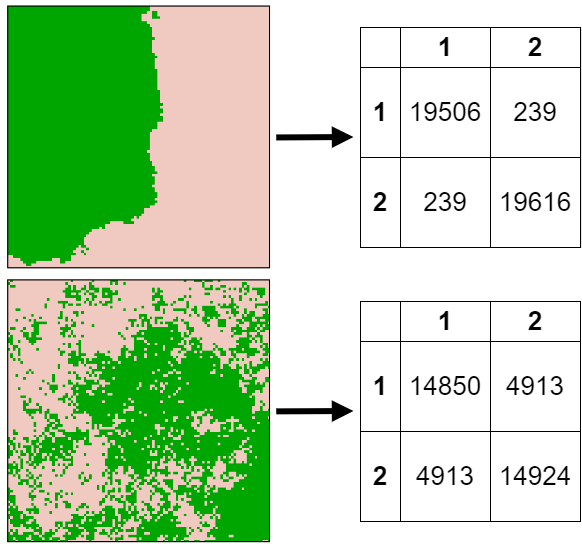
\includegraphics[width=3.64583in,height=3.64583in]{figures/diagram_coma.png}

}

\caption{\label{fig-metody-coma}Przykład dwóch macierzy
współwystępowania dla rastrów o zbliżonej kompozycji i różnej
konfiguracji przestrzennej.}

\end{figure}

W celu porównywania ze sobą sygnatur dwóch rastrów w postaci
dwuwymiarowej macierzy należy je sprowadzić do postaci jednowymiarowych
wektorów (histogramów), a następnie przeprowadzić ich normalizację, tak
aby wszystkie wartości sumowały się do 1. Taka postać umożliwia
obliczanie miar odległości lub podobieństwa, pozwalających na
porównywanie histogramów wartości \autocite{Cha2007}. Miary te następnie
pozwalają określić stopień odmienności dwóch rastrów. Podejście to może
być także wykorzystane w innych analizach przestrzennych, jak
wyszukiwanie obszarów o podobnej strukturze przestrzennej, grupowanie
tych obszarów oraz wykrywanie ich zmian
\autocite{Jasiewicz_GeoPAT,nowosad_motif}.

\hypertarget{miary-wywodzux105ce-siux119-z-teorii-informacji}{%
\section{Miary wywodzące się z teorii
informacji}\label{miary-wywodzux105ce-siux119-z-teorii-informacji}}

Metodologia, którą w pracy \textcite{nowosad_it} zakłada, że
podstawowymi jednostkami analizy dla miar wywodzących się z teorii
informacji nie są poszczególne komórki rastra, lecz pary sąsiadujących
komórek. Parą natomiast określa się dwuwartościową zmienną losową
(\(x\), \(y\)), dla której \(x\) reprezentuje klasę analizowanej
komórki, a \(y\) jest klasą sąsiedniej komórki. Zmienna (\(x\), \(y\))
przyjmuje wartości (\(c_i\), \(c_j\)), które mieszczą się w zakresie od
1 do \(K\), gdzie \(K\) reprezentuje liczbę klas obecnych na rastrze. Na
tej podstawie, macierz współwystępowania może być traktowana jako
dwuwymiarowy histogram par komórek, w którym każdy przedział wskazuje
liczbę par (\(c_i\), \(c_j\)).

W tej pracy wykorzystane zostały dwie miary z teorii informacji.
Pierwszą jest entropia brzegowa (ang. marginal entropy). Opisuje ona
zróżnicowanie kompozycji rastra, czyli udziałów każdej z kategorii w
rastrze. Im wyższa wartość tej miary, tym bardziej zróżnicowane są
poszczególne klasy. Entropia brzegowa może być obliczona zgodnie ze
wzorem:

\[H(y) = -\sum_{j=1}^{K}p(y=c_{j})log_2p(y=c_j)\]

\begin{itemize}
\item
  \(K\) - liczba kategorii pokrycia terenu
\item
  \(p(y = c_j)\) - prawdopodobieństwo, że sąsiadująca komórka \(y\) ma
  przypisaną klasę \(c_j\)
\end{itemize}

Drugą miarą, która została wykorzystana w tej pracy jest względna
informacja wzajemna (ang. relative mutual information). Opisuje ona
stopień sąsiadowania ze sobą kategorii w rastrze, czyli jego
konfigurację przestrzenną. Względna informacja wzajemna przyjmuje
wartości w zakresie od 0 do 1. Im niższa wartość tej miary, tym bardziej
pofragmentowany jest cały krajobraz. Względną informację wzajemną można
obliczyć ze wzoru: \[U = I(y,x)/H(y)\] gdzie \(I(y,x)\) oznacza
informację wzajemną, liczoną ze wzoru: \[I(y,x) = H(y) - H(y|x)\]
natomiast \(H(y|x)\) reprezentuje entropię warunkową, obliczaną zgodnie
ze wzorem:
\[H(y|x) = \sum_{i=1}^{K}\sum_{j=1}^{K} p(x=c_i, y=c_j) log_2 p(y=c_i | x=c_j)\]

\begin{itemize}
\item
  \(p(x=c_i, y=c_j)\) - prawdopodobieństwo, że analizowana komórka \(x\)
  jest klasy \(c_i\) oraz sąsiadująca komórka \(y\) jest klasy \(c_j\)
\item
  \(p(y=c_i | x=c_j)\) - prawdopodobieństwo, że komórka \(y\) jest klasy
  \(c_i\) pod warunkiem, że analizowana komórka jest klasy \(c_j\)
\end{itemize}

\hypertarget{sec-pattern-based}{%
\section{Metody analiz różnic pokrycia terenu}\label{sec-pattern-based}}

Zmiany pokrycia terenu w czasie lub różnice w pokryciu terenu pomiędzy
obrazami można analizować przy użyciu wielu metod. Wiele z nich
koncentruje się na analizie różnic na poziomie indywidualnych komórek w
siatce rastra. Najbardziej podstawowym przykładem takiego podejścia jest
analiza ilościowa różnic w pokryciu terenu. Zaletą tego podejścia jest
przede wszystkim łatwość w wykonaniu analizy. Wystarczy zliczyć
wszystkie komórki należące do poszczególnych kategorii dla wybranych
rastrów, a następnie porównać ze sobą te wartości, aby otrzymać wynik
informujący nas o ilościowych różnicach między analizowanymi rastrami.
Analiza ilościowa najczęściej wykorzystywana jest w celu wskazania
ogólnych trendów zmian pokrycia terenu dla określonego obszaru badań jak
na przykład zmniejszanie się obszarów leśnych lub wzrost terenów
zurbanizowanych.

Wszelkie metody analiz zmian pokrycia terenu opierające się na analizie
poszczególnych komórek w siatce rastra są użyteczne na obszarach, gdzie
zmiany między indywidualnymi komórkami dostarczają istotnych informacji.
Ich przydatność jednak maleje, gdy informacja na poziomie pojedynczej
komórki przestaje być tak istotna, na przykład dla rastrów o wysokiej
rozdzielczości lub znacznym zasięgu przestrzennym
\autocite{Jasiewicz_GeoPAT}. W takiej sytuacji bardziej efektywne staje
się zastosowanie metod opartych na analizie struktur przestrzennych
(ang. pattern-based change assessment) \autocite{Netzel2015}.

Pozwalają one przede wszystkim na opis oraz obliczenie podobieństwa
struktur przestrzennych. Głównym zamysłem tych metod jest
przekształcenie danych z postaci dużych rastrów zbudowanych z wielu
indywidualnych komórek zawierających pojedyncze informacje w metryki
krajobrazowe oraz sygnatury przestrzenne, a następnie porównanie ich za
pomocą miar odległości lub niepodobieństwa. Zastosowanie metryk
krajobrazowych w kontekście kompleksowych analiz przestrzennych ma
jednak istotną wadę. Jako że pojedyncza metryka krajobrazowa
reprezentuje wyłącznie jedną, konkretną charakterystykę analizowanego
obszaru, to nie jest w stanie opisać całej charakterystyki struktury
przestrzennej danego rastra. W tym celu korzystniejsze może okazać się
zastosowanie sygnatur przestrzennych. Dzięki temu, że są dwuwymiarową
reprezentacją struktury przestrzennej rastrów, można je porównywać ze
sobą przy użyciu szerokiej gamy istniejących miar odległości i
niepodobieństwa.

\hypertarget{miary-odlegux142oux15bci-i-niepodobieux144stwa}{%
\section{Miary odległości i
niepodobieństwa}\label{miary-odlegux142oux15bci-i-niepodobieux144stwa}}

Odległość oraz rozbieżność (inaczej niepodobieństwo) stanowią pewien
policzalny stopień różnorodności pary obiektów. Największą różnicą
między nimi jest to, że odległości są symetryczne, podczas gdy
rozbieżności są niesymetryczne. Oznacza to, że wyłącznie dla miar
odległości otrzymujemy identyczny wynik przy porównywaniu par obiektów A
i B, jak i par B i A.

Rozbieżność jest przeciwieństwem podobieństwa. Ponadto, miary
podobieństwa można łatwo przekształcić w miary niepodobieństwa
\autocite{niesterowicz2016}. W związku z tym, w celu uproszczenia
terminologii, wszystkie miary odległości, podobieństwa oraz te wywodzące
się z dziedziny teorii informacji, które zostały wykorzystane w tej
pracy, będą dalej zbiorowo nazywane miarami niepodobieństwa.

Na podstawie podobieństw syntaktycznych, wyróżnia się kilka grup rodzin
miar niepodobieństwa \autocite{Cha2007}: rodzina Minkowski (odległość
euklidesowa, odległość Minkowskiego, odległość Manhattan), rodzina
\(L_1\) (Canberra, Sorensen, Kulczynski), rodzina Intersection
(Intersection, Wave Hedges, Ruzicka), rodzina Inner Product (Jaccard,
Harmonic mean), rodzina Squared-chord (Fidelity, Matusita), rodzina
\(\chi^2\) (Clark, Pearson \(\chi^2\), Neyman \(\chi^2\)), rodzina
Shannon's Entropy (Jensen-Shannon, Kullback-Leibler), a także miary
będące połączeniem innych miar (Taneja, Kumar-Johnson) oraz miary
wywodzące się z teorii informacji (informacja wzajemna, entropia
Shannona). Wybór odpowiedniej miary niepodobieństwa zależy między innymi
od rodzaju pomiaru lub sposobu reprezentacji obiektów
\autocite{Cha2007}.

\hypertarget{obliczenie-niepodobieux144stwa-rastruxf3w}{%
\section{Obliczenie niepodobieństwa
rastrów}\label{obliczenie-niepodobieux144stwa-rastruxf3w}}

Pierwszym krokiem, jaki należy podjąć w celu obliczenia podobieństwa
struktur przestrzennych danych rastrowych z wykorzystaniem metod
opartych o sygnatury przestrzenne jest sprowadzenie rastrów wejściowych
do postaci macierzy współwystępowania. Proces utworzenia macierzy
współwystępowania polega na zliczeniu wartości każdej indywidualnej
komórki rastra, a także przylegających do niej komórek (najczęściej
czterech lub ośmiu). Przykładowe macierze współwystępowania widoczne są
na Rycinie \ref{fig-metody-coma}. Następnie, dwuwymiarową macierz należy
sprowadzić do postaci jednowymiarowej, czyli wektora współwystępowania.
Kolejnym etapem analizy jest normalizacja wektora współwystępowania. Po
dodaniu do siebie wszystkich wartości tego wektora powinniśmy otrzymać
wynik równy 1. Po wykonaniu powyższych czynności otrzymujemy
reprezentację rastrów wejściowych, która umożliwia porównanie ich ze
sobą przy użyciu miar niepodobieństwa między rozkładami
prawdopodobieństwa, takich jak rozbieżność Jensena-Shannona. Proces
obliczenia niepodobieństwa dwóch rastrów w postaci schematu przedstawia
Rycina \ref{fig-schemat-porownanie}.

\begin{figure}[t]

{\centering 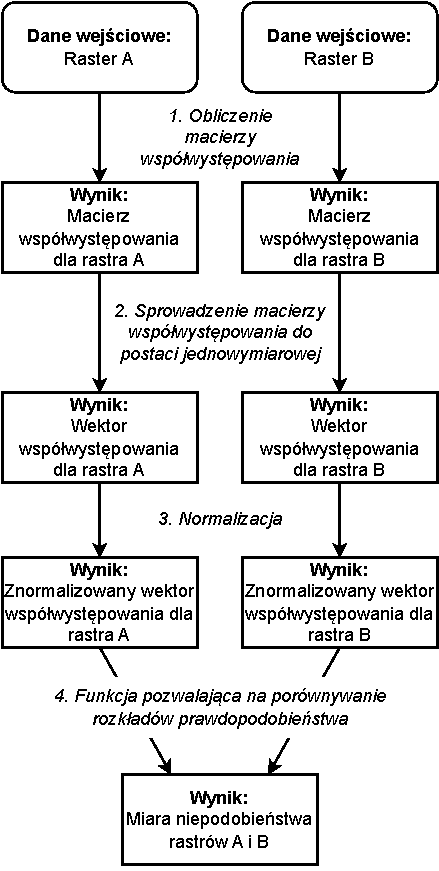
\includegraphics[width=4.19792in,height=8.33333in]{figures/diagram_raster_comparison.pdf}

}

\caption{\label{fig-schemat-porownanie}Schemat procesu obliczenia
niepodobieństwa dwóch rastrów.}

\end{figure}

\bookmarksetup{startatroot}

\hypertarget{sec-materialy}{%
\chapter{Materiały}\label{sec-materialy}}

W pierwszej kolejności w tym rozdziale są omawiane aspekty związane z
formą przeprowadzonej ankiety. Przedstawiony jest proces symulacji,
który został wykorzystany do stworzenia zbioru danych o określonych
parametrach kompozycji i konfiguracji przestrzennej. Następnie opisany
jest sposób doboru pytań do ankiety. W końcowej części rozdziału są
omówione dane przestrzenne o pokryciu terenu CORINE Land Cover, które
zostały wykorzystane do porównania stosowania wybranych miar
niepodobieństwa w kontekście analiz zmian pokrycia terenu.

\hypertarget{sec-symulowanie}{%
\section{Symulowanie rastrów o określonej kompozycji i konfiguracji
przestrzennej}\label{sec-symulowanie}}

Najważniejszym założeniem przy tworzeniu zbioru rastrów do ankiety było
przygotowanie ich w sposób umożliwiający uzyskanie pełnej reprezentacji
wszystkich możliwych wartości kompozycji, jak i konfiguracji
przestrzennej. Zbiór rastrów został przygotowany w języku programowania
R \autocite{R2023}, w oparciu o wykorzystanie funkcji \emph{nlm\_fbm} z
pakietu NLMR \autocite{NLMR2018}. Powyższa funkcja umożliwia uzyskanie
danych rastrowych wypełnionych wartościami zmiennoprzecinkowymi
mieszczącymi się w zakresie od 0 do 1 oraz dowolnymi parametrami
konfiguracji przestrzennej. Funkcja ta pozwala na symulację rastrów przy
użyciu ułamkowych ruchów Browna, będących uproszczeniem ruchów Browna
\autocite{nlm_fbm}. W tej funkcji poziom autokorelacji między kolejnymi
symulacjami jest kontrolowany za pomocą parametru wymiaru fraktalnego
(``fract\_dim''). W kontekście tego badania, parametr ten reguluje
konfigurację przestrzenną. Oznacza to, że w przypadku, gdy
``fract\_dim'' przyjmuje niską wartość, zbliżoną do 0, wartości w
generowanym rastrze rozmieszczone są w sposób losowy, zbliżony do szumu.
Natomiast w przypadku wysokiej wartości ``fract\_dim'', zbliżonej do 2,
na wynikowym rastrze tworzą się skupiska najwyższych i najniższych
wartości, a przejścia pomiędzy nimi mają płynny, wygładzony charakter.

Następnie, aby otrzymać zbiór rastrów uwzględniający także pełen
przekrój kompozycji należy przeprowadzić proces reklasyfikacji rastrów
stworzonych w poprzednim kroku. Procedura ta polega na podziale każdego
dotychczas utworzonego rastra na kategorie pokrycia terenu w różnych
proporcjach, na przykład 90:10, 70:30 oraz 50:50 w przypadku rastrów
zawierających wyłącznie dwie kategorie pokrycia terenu. Wykonanie tego
procesu ułatwia funkcja \emph{util\_binarize} z pakietu landscapetools
\autocite{NLMR2018}. W tej funkcji proporcje kategorii pokrycia terenu
kontrolowane są za pomocą parametru ``breaks''. Przykładowo, ustawienie
parametru ``breaks'' na poziomie \emph{0.2} poskutkuje otrzymaniem
rastra o kategoriach pokrycia terenu w proporcjach 20 do 80. Oznacza to,
że jedna z kategorii będzie pokrywała 20\% komórek rastra, podczas gdy
druga kategoria wypełni pozostałe 80\% komórek. Na Rycinie
\ref{fig-diagram-symulowanie} przedstawiony został przykład
przygotowania rastrów podzielonych na dwie kategorie pokrycia terenu w
sposób opisany powyżej.

\begin{figure}[t]

{\centering 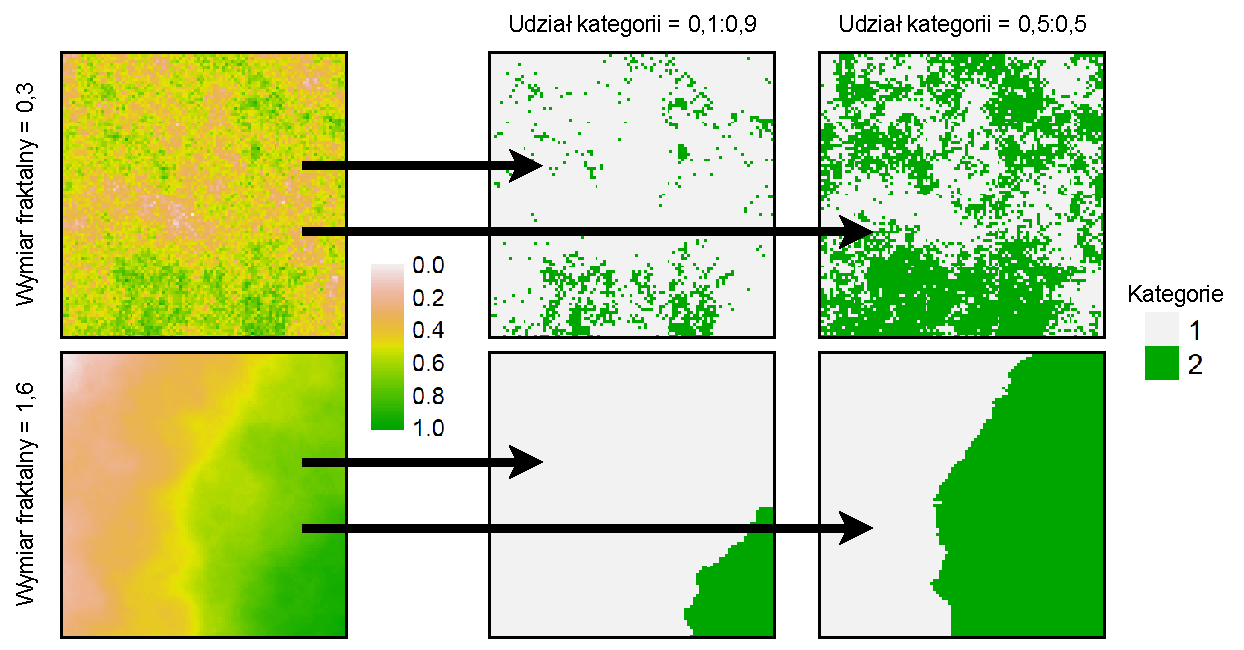
\includegraphics[width=5.20833in,height=2.70833in]{figures/diagram_rastersim_showcase.pdf}

}

\caption{\label{fig-diagram-symulowanie}Symulowanie rastrów o określonej
kompozycji i konfiguracji przestrzennej}

\end{figure}

Ostatecznie wygenerowane zostały zbiory rastrów składających się
wyłącznie z dwóch lub trzech kategorii pokrycia terenu. Przykład jednego
ze zbiorów rastrów przedstawia Rycina \ref{fig-wykres1_2classes}. Rastry
zawierające trzy kategorie zostały uwzględnione w badaniu w celu próby
wskazania czy liczba kategorii na rastrach ma wpływ na odpowiedzi
udzielane przez ankietowanych.

Po utworzeniu zbioru danych rastrowych bardzo istotne było
potwierdzenie, że obejmuje on pełen zakres rozkładu kompozycji i
konfiguracji. Na potwierdzenie tego założenia pozwoliło obliczenie
wybranych miar opisujących struktury przestrzenne: entropii oraz
względnej informacji wzajemnej.

\begin{figure}[t]

{\centering 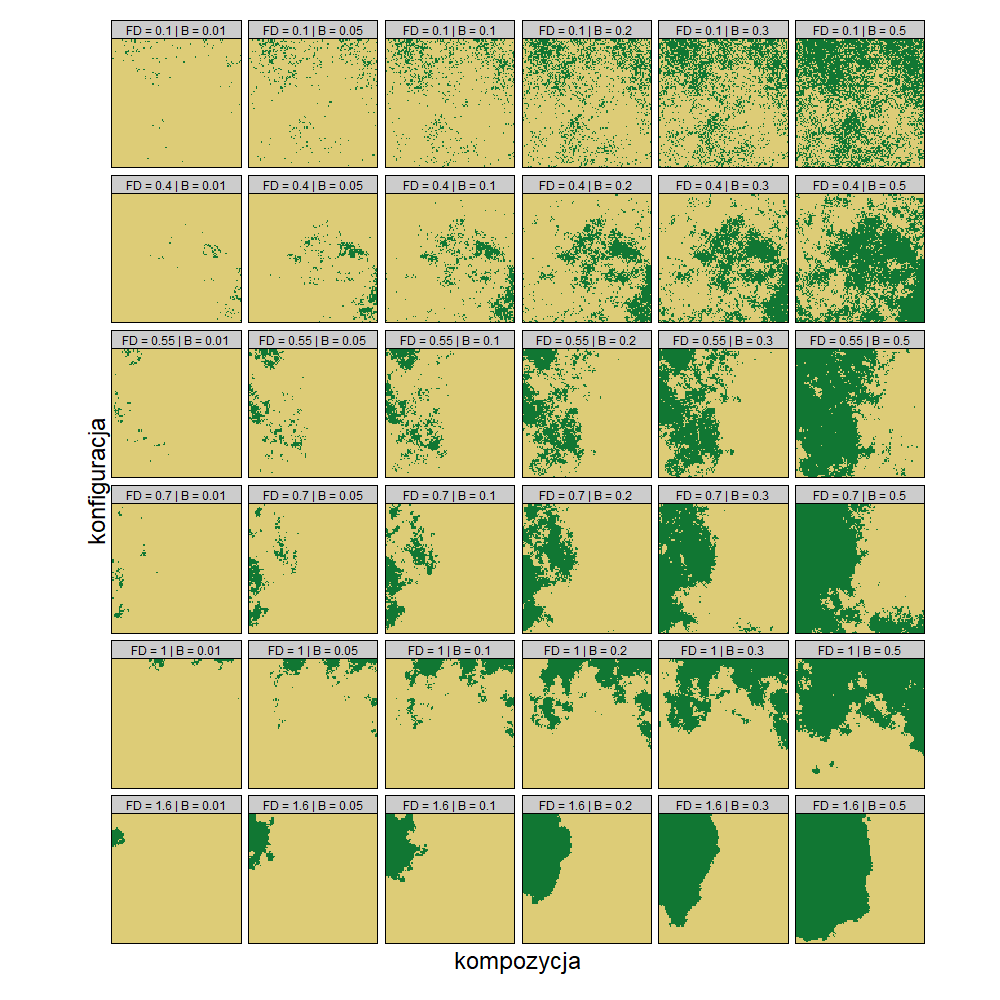
\includegraphics[width=5.72917in,height=5.72917in]{figures/wykres1_2classes.png}

}

\caption{\label{fig-wykres1_2classes}Przykład zbioru wygenerowanych
rastrów (2 kategorie pokrycia terenu)}

\end{figure}

\hypertarget{sec-przygotowanie1}{%
\section{Przygotowanie ankiety}\label{sec-przygotowanie1}}

Ostatnim krokiem przygotowania danych do ankiety było wybranie par
rastrów tworzących poszczególne pytania, tak aby uwzględniały one
wszelkie możliwe różnice struktury przestrzennej rastrów. W tym celu,
pytania w ankietach podzielone zostały na dwie grupy, wewnątrz których
znalazły się po trzy podgrupy pytań.

W pierwszej kolejności respondenci zetknęli się z 24 pytaniami
dotyczącymi rastrów uwzględniających wyłącznie dwie kategorie pokrycia
terenu, a następnie z 24 pytaniami uwzględniającymi trzy kategorie
pokrycia terenu. Pierwsza podgrupa pytań (6 par rastrów) składała się z
par rastrów różniących się między sobą wyłącznie entropią. Podgrupa
druga (6 par rastrów) zawierała wyłącznie rastry różniące się względną
informacją wzajemną. Ostatnia podgrupa (12 par rastrów) składała się z
pytań zróżnicowanych zarówno pod względem entropii, jak i względnej
informacji wzajemnej.

Taki sposób doboru pytań pozwolił na zredukowanie liczby odpowiedzi
wymaganych od respondentów, jak i ograniczenie wpływu błędu selekcji,
który powstałby w wyniku niewłaściwego doboru pytań. Respondenci celowo
nie zostali poinformowani o występujących różnicach pomiędzy kolejnymi
pytaniami, ponieważ mogłoby mieć to wpływ na udzielane przez nich
odpowiedzi, co z kolei mogłoby wpłynąć na ostateczne wyniki badania.

\hypertarget{sec-CLC}{%
\section{Dane CORINE Land Cover}\label{sec-CLC}}

Jednym z etapów pracy było zastosowanie uzyskanych wcześniej wyników do
analizy zmian pokrycia terenu na podstawie danych CORINE Land Cover
(CLC). Dane CLC reprezentują szczegółowe informacje o pokryciu terenu,
klasyfikując obszary według różnych kategorii, takich jak lasy, tereny
rolnicze, obszary zurbanizowane czy zbiorniki wodne. Stanowią one
istotny instrument w analizie i monitorowaniu zmian środowiska, a także
służą jako narzędzie wspierające procesy decyzyjne na poziomie
europejskim.

Zbiory danych przestrzennych CORINE Land Cover stanowią integralną część
programu CORINE (Coordination of Information on Environment),
wprowadzonego przez Komisję Wspólnot Europejskich w 1985 roku. Program
ten został stworzony w celu skoordynowania przedsięwzięć związanych z
gromadzeniem i przetwarzaniem informacji na temat stanu środowiska
geograficznego w krajach należących do Wspólnoty Europejskiej oraz
standaryzację tych danych w celu ułatwienia wymiany informacji między
państwami członkowskimi \autocite{Bielecka_Ciolkosz_2004}.

Wyniki programu CORINE są udostępniane w formatach wektorowych ESRI i
SQLite geodatabase oraz formacie rastrowym GeoTiff o rozdzielczości
przestrzennej 100 metrów, co oznacza, że jedna komórka rastra obejmuje 1
hektar powierzchni. Do celów tej pracy, wykorzystane zostały dane CLC
dla lat 1990 i 2018 udostępnione do pobrania w formacie GeoTiff na
witrynie Copernicus Land Monitoring Service
(https://land.copernicus.eu/pan-european/corine-land-cover). Dane te
wykorzystują układ współrzędnych ETRS-LAEA (EPSG:3035).

Dane CLC są zorganizowane na trzech poziomach szczegółowości. Na
najwyższym poziomie tej hierarchii wyodrębniono pięć głównych typów
pokrycia terenu: tereny antropogeniczne, tereny rolne, lasy i ekosystemy
seminaturalne, obszary podmokłe oraz obszary wodne. W celu uproszczenia
analizy wyników, dane zostały poddane reklasyfikacji. W wyniku tego
procesu zredukowano liczbę kategorii pokrycia terenu do wyłącznie dwóch:
lasy i pozostałe obszary.

\bookmarksetup{startatroot}

\hypertarget{sec-wyniki}{%
\chapter{Wyniki ankiety}\label{sec-wyniki}}

Niniejszy rozdział przedstawia kompleksowe podsumowanie oraz analizę
wyników przeprowadzonej ankiety. W pierwszej kolejności omówione są
ogólne informacje dotyczące samej ankiety, takie jak termin jej
przeprowadzenia, profil respondentów oraz sposób realizacji badania.
Przedstawione jest podsumowanie wyników ankiety, obejmujące między
innymi liczbę udzielonych odpowiedzi poszczególnych typów oraz wskazanie
poziomów zgodności podgrup pytań. Kolejnym opisanym aspektem są miary
niepodobieństwa wykorzystane w badaniu oraz analiza relacji między tymi
miarami a różnymi sposobami podsumowania odpowiedzi. Dalsza analiza
koncentruje się na badaniu związku między średnią odpowiedzią a miarami
niepodobieństwa, w podziale na grupy pytań uwzględniające dwie oraz trzy
kategorie pokrycia terenu. Końcowa część rozdziału skupia się na
analizie relacji między odpowiedziami a różnicami między miarami z
teorii informacji.

\hypertarget{podsumowanie-ankiety}{%
\section{Podsumowanie ankiety}\label{podsumowanie-ankiety}}

W celu zidentyfikowania potencjalnych związków pomiędzy percepcją zmian
w pokryciu terenu przez ludzi a miarami niepodobieństwa, które te zmiany
kwantyfikują przeprowadzona została ankieta. Głównym celem ankiety było
uzyskanie wstępnych informacji na temat tego w jaki sposób różnice w
entropii oraz względnej informacji wzajemnej między analizowanymi
rastrami wpływają na subiektywne postrzeganie zmian w pokryciu terenu
przez ludzi.

Badanie było realizowane w terminie od 21 do 24 listopada 2022 roku. Z
uwagi na znaczną liczbę rastrów, które miałyby być przedstawione
ankietowanym w trakcie badania, proces zbierania odpowiedzi respondentów
przyjął formę ankiety internetowej. Pozwoliło to respondentom na wygodny
udział w badaniu przy użyciu komputera lub urządzenia mobilnego.
Kwestionariusz stworzony został w formie aplikacji internetowej za
pomocą języka programowania R, na podstawie pakietów shiny
\autocite*{R-shiny} oraz shinysurveys \autocite*{R-shinysurveys}. Sama
aplikacja umieszczona została na platformie \emph{shinyapps.io}
(https://www.shinyapps.io/). Przeprowadzenie ankiety w tej formie
umożliwiło systematyczne gromadzenie oraz przechowywanie odpowiedzi w
formie tabelarycznej, ułatwiając tym samym dalszą analizę i
interpretację danych. Respondenci stanowili grupę 50 studentów drugiego
i trzeciego roku studiów inżynierskich na kierunku Geoinformacja na
Wydziale Nauk Geograficznych i Geologicznych Uniwersytetu im. Adama
Mickiewicza. Wybór tej grupy respondentów oznacza, że byli oni już
zaznajomieni z tematyką tworzenia i analiz map w formie rastrowej oraz
pojęciem zmian pokrycia terenu.

Każdy z ankietowanych otrzymał do wypełnienia jeden z dwóch wcześniej
przygotowanych zbiorów pytań. Każdy ze zbiorów składał się z 48 pytań,
przy czym część pytań między zbiorami się pokrywała. Oznacza to, że
łącznie uzyskano odpowiedzi na 93 unikatowe pytania. W każdym z pytań
zadaniem respondentów było określenie podobieństwa na podstawie dwóch
załączonych rastrów. W ramach badania respondenci mieli możliwość
wyrażania swoich odpowiedzi za pomocą pięciostopniowej skali Likerta
\autocite{likert_scale}, która obejmowała poziomy podobieństwa od
``Brak'' przez ``Bardzo małe'', ``Umiarkowane'', ``Bardzo duże'' aż po
``Pełne''. Wykorzystanie skali Likerta o nieparzystej liczbie
przedziałów, pozwoliło na zastosowanie przedziału środkowego, którego
celem było reprezentowanie odpowiedzi neutralnych lub trudnych do
określenia. Początkowo, zamiast skali Likerta planowano wykorzystać
skalę liczbową, w zakresie mieszczącym się od 1 do 100, jednakże
zrezygnowano z tego pomysłu, jako że znaczenie wartości na skali
liczbowej może być interpretowane inaczej przez każdego respondenta oraz
skala ta nie pozwala na uwzględnienie wspomnianej wcześniej odpowiedzi
neutralnej. Przykład pytania przedstawionego respondentom ilustruje
Rycina \ref{fig-przyklad_pytania}.

\begin{figure}[t]

{\centering 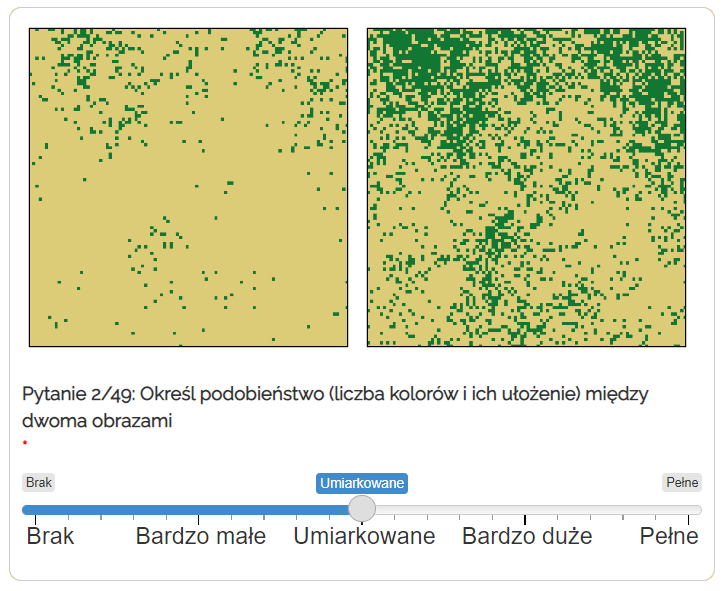
\includegraphics[width=5.10417in,height=4.16667in]{figures/przyklad_pytania.png}

}

\caption{\label{fig-przyklad_pytania}Przykładowe pytanie z ankiety}

\end{figure}

Łącznie uzyskano 2400 odpowiedzi. Ich podsumowanie przedstawione zostało
w Tabeli \ref{tbl-totals_df}. Według ankietowanych prawie 36\% par
rastrów charakteryzowała się brakiem podobieństwa, 32,6\% uzyskanych
odpowiedzi wskazywało na bardzo małe podobieństwo, 18,1\% na
umiarkowane, 11,6\% bardzo duże, natomiast mniej niż 2\% wskazywało na
pełne podobieństwo. Warto tutaj także zwrócić uwagę, że zestawienia
wszystkich odpowiedzi w zależności od liczby kategorii widocznych na
rastrach nie wskazują na znaczące różnice w liczbie odpowiedzi dla danej
kategorii. Największą różnicę stanowi w tym przypadku kategoria ``Bardzo
duże'', dla której liczba odpowiedzi dla rastrów z dwoma i trzema
kategoriami pokrycia terenu różni się zaledwie o 2,7\%. Najmniejszą
różnicą charakteryzuje się kategoria ``Pełne'', gdzie liczba odpowiedzi
pomiędzy zestawami różni się o jedyne 0,9\%.

\hypertarget{tbl-totals_df}{}
\begin{table}
\caption{\label{tbl-totals_df}Podsumowanie odpowiedzi z ankiety }\tabularnewline

\centering
\begin{tabular}{>{\raggedright\arraybackslash}p{3cm}>{\raggedleft\arraybackslash}p{2.5cm}>{\raggedleft\arraybackslash}p{2.5cm}>{\raggedleft\arraybackslash}p{2.5cm}}
\toprule
Typ odpowiedzi & Łącznie & Dwie klasy & Trzy klasy\\
\midrule
Brak & 862 & 420 & 442\\
Bardzo małe & 783 & 398 & 385\\
Umiarkowane & 434 & 211 & 223\\
Bardzo duże & 278 & 155 & 123\\
Pełne & 43 & 16 & 27\\
\addlinespace
Suma & 2400 & 1200 & 1200\\
\bottomrule
\end{tabular}
\end{table}

\hypertarget{poziom-zgodnoux15bci-ankietowanych}{%
\section{Poziom zgodności
ankietowanych}\label{poziom-zgodnoux15bci-ankietowanych}}

Aby określić jakie odpowiedzi należały do grupy najczęstszych odpowiedzi
dla poszczególnych pytań, obliczona została miara określana dalej
``poziomem zgodności''. Poziom zgodności każdego pytania został
obliczony jako stosunek najczęściej udzielonej odpowiedzi względem
całkowitej liczby odpowiedzi udzielonych na to pytanie.

Poziomy zgodności ankietowanych w podziale na rodzaje pytań znajdują się
w Tabeli \ref{tbl-qtype_agree_df1}. Całkowity poziom zgodności
ankietowanych został oszacowany na 55\%. Oznacza to, że 1321 z 2400
udzielonych odpowiedzi znalazło się w grupie najczęściej udzielonych
odpowiedzi na pytania. Pytania zawierające rastry różniące się zarówno
entropią, jak i względną informacją wzajemną cechowały się najwyższym
poziomem zgodności odpowiedzi wynoszącym 61\%, podczas gdy pytania
różniące się wyłącznie entropią uzyskały wynik 53\%, a pytania różniące
się wyłącznie względną informacją wzajemną uzyskały wynik 52\%.

\hypertarget{tbl-qtype_agree_df1}{}
\begin{table}
\caption{\label{tbl-qtype_agree_df1}Poziom zgodności ankietowanych w podziale na rodzaje pytań }\tabularnewline

\centering
\begin{tabular}{>{\raggedright\arraybackslash}p{4cm}>{\raggedleft\arraybackslash}p{3cm}>{\raggedleft\arraybackslash}p{3cm}>{\raggedleft\arraybackslash}p{3cm}}
\toprule
Podgrupa pytań & Liczba najczęstszych odpowiedzi & Liczba odpowiedzi & Poziom zgodności [\%]\\
\midrule
Różna entropia, różna RMI & 429 & 704 & 61\\
Różna entropia, identyczna RMI & 425 & 796 & 53\\
Identyczna entropia, identyczna RMI & 467 & 900 & 52\\
Łącznie & 1321 & 2400 & 55\\
\bottomrule
\multicolumn{4}{l}{\rule{0pt}{1em}RMI - względna informacja wzajemna}\\
\end{tabular}
\end{table}

Najwyższy poziom zgodności odpowiedzi osób ankietowanych wyniósł 92\% i
dotyczył pytania różniącego się zarówno entropią, jak i względną
informacją wzajemną. Aż 24 z 26 osób wskazało na brak podobieństw między
rastrami uwzględnionymi w tym pytaniu. Jest to interesujący wynik,
ponieważ rastry w tym pytaniu wcale nie należały do par rastrów
najbardziej zróżnicowanych pod względem entropii i względnej informacji
wzajemnej. Pierwszy z rastrów charakteryzował się entropią na poziomie
0,08 oraz względną informacją wzajemną wynoszącą 0,09. W przypadku
drugiego rastra, wspomniane wartości wynosiły odpowiednio 0,47 i 0,48.
Oznacza to, że w przypadku obu miar różnica między parami entropii oraz
wynikami względnej informacji wzajemnej wyniosły 0,39.

\textbf{\emph{RYCINA RYCINA RYCINA RYCINA RYCINA RYCINA RYCINA RYCINA }}

Najniższy poziom zgodności, czyli zaledwie 38\%, osiągnęło aż 8 pytań.
Wyłącznie dwa z nich dotyczyły pytań zawierających trzy kategorie
pokrycia terenu. 75\% z tych pytań uwzględniało rastry różniące się pod
względem względnej informacji wzajemnej (różna konfiguracja) przy
zachowaniu tej samej entropii (identyczna kompozycja).

\hypertarget{miary-niepodobieux144stwa}{%
\section{Miary niepodobieństwa}\label{miary-niepodobieux144stwa}}

Do analizy relacji między miarami niepodobieństwa a wynikami ankiety
wybrano 20 miar niepodobieństwa, za pomocą których zostało obliczone
niepodobieństwo każdej pary rastrów uwzględnionych w ankiecie.
Uwzględnione zostały wyłącznie miary, których wyniki dla zbiorów rastrów
nie wykazały bardzo silnego podobieństwa z wynikami innych miar. Decyzja
ta pozwoliła skoncentrować się na bardziej zróżnicowanym zestawie miar
niepodobieństwa, \textbf{\emph{natomiast podobne teoretycznie miary mają
swoich przedstawicieli wśród uwzględnionych miar.}}

W analizie uwzględniono miary: Addytywne \(\chi^2\), odległość Canberra,
Czebyszewa, Clarka, Hellingera, iloczyn skalarny, Jaccarda,
Jensena-Shannona, Kullbacka-Leiblera, Kumara-Hassebrooka,
Kumara-Johnsona, odległość Manhattan, Neymana, odległość euklidesową,
Pearsona, podobieństwo cosinusowe (Cosinus), Ruzicki, Tanejy, średnią
harmoniczną oraz Wave Hedgesa.

\hypertarget{odpowiedzi-i-miary-niepodobieux144stwa}{%
\section{Odpowiedzi i miary
niepodobieństwa}\label{odpowiedzi-i-miary-niepodobieux144stwa}}

Analizę relacji między odpowiedziami a miarami niepodobieństwa
rozpoczęto od obliczenia korelacji między różnymi sposobami podsumowania
odpowiedzi a miarami niepodobieństwa. W tym celu, oryginalna skala
odpowiedzi z ankiety, która obejmowała wartości od ``Brak'' do
``Pełne'', została przekształcona na skalę liczbową. W tym procesie
odpowiedzi ``Brak'' została przypisana wartość 5, a każdej kolejnej
odpowiedzi została przyporządkowana niższa cyfra, aż do ``Pełne'',
której przypisano wartość 1.

Pod uwagę wzięto cztery sposoby podsumowania odpowiedzi: średnią z
odpowiedzi, medianę odpowiedzi, najczęstszą odpowiedź (modę) oraz
odchylenie standardowe (SD). Następnie współczynnik korelacji Spearmana,
którego zakres wartości mieści się między -1 a 1 został przeliczony na
współczynnik determinacji \(R^2\), którego wartości oscylują w zakresie
od 0 do 1. Relacja wyników danej miary z odpowiedziami ankietowanych
jest tym silniejsza, im bliższa 1 jest wartość współczynnika
determinacji.

\hypertarget{tbl-mc2_cors}{}
\begin{table}
\caption{\label{tbl-mc2_cors}Zestawienie wskaźników korelacji Spearmana wybranych metod podsumowania
odpowiedzi dla 2 klas }\tabularnewline

\centering
\begin{tabular}{lrrrr}
\toprule
Sposób podsumowania
odpowiedzi & Średnia & Mediana & Moda & SD\\
\midrule
Średnia & 1.00 & 0.93 & 0.86 & 0.37\\
Mediana & 0.93 & 1.00 & 0.90 & 0.23\\
Moda & 0.86 & 0.90 & 1.00 & 0.06\\
SD & 0.37 & 0.23 & 0.06 & 1.00\\
\bottomrule
\end{tabular}
\end{table}

\hypertarget{tbl-mc3_cors}{}
\begin{table}
\caption{\label{tbl-mc3_cors}Zestawienie wskaźników korelacji Spearmana wybranych metod podsumowania
odpowiedzi dla 3 klas }\tabularnewline

\centering
\begin{tabular}{lrrrr}
\toprule
Sposób podsumowania
odpowiedzi & Średnia & Mediana & Moda & SD\\
\midrule
Średnia & 1.00 & 0.93 & 0.89 & 0.32\\
Mediana & 0.93 & 1.00 & 0.91 & 0.17\\
Moda & 0.89 & 0.91 & 1.00 & 0.11\\
SD & 0.32 & 0.17 & 0.11 & 1.00\\
\bottomrule
\end{tabular}
\end{table}

Zarówno w przypadku rastrów z dwoma (Tabela \ref{tbl-mc2_cors}) i trzema
klasami (Tabela \ref{tbl-mc3_cors}) średnia, mediana i moda odpowiedzi
są ze sobą silnie skorelowane oraz wszystkie mają względnie niewielką,
ale widoczną korelację z odchyleniem standardowym odpowiedzi. Najwyższą
wartość współczynnika korelacji z odchyleniem standardowym ma średnia
odpowiedzi (0,37).

\begin{figure}[t]

{\centering 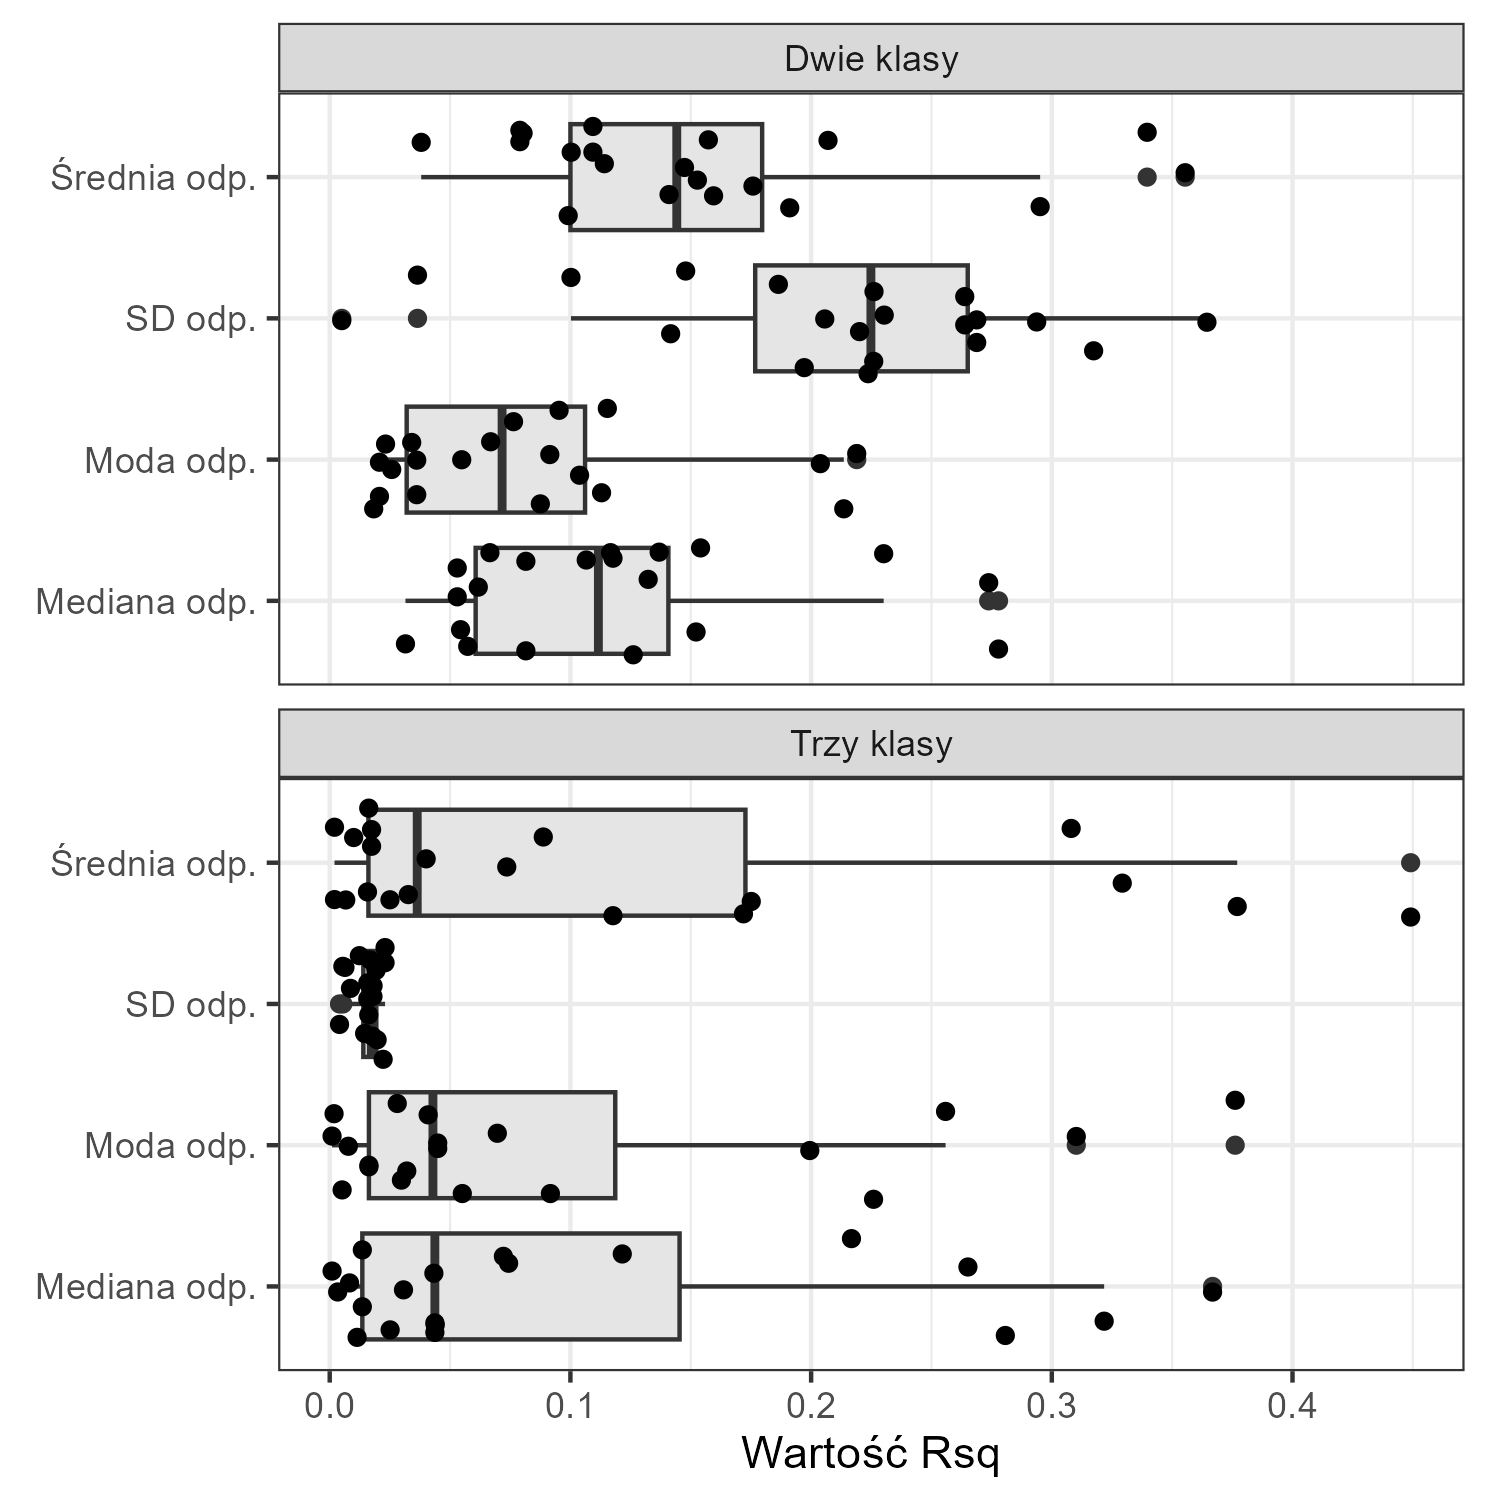
\includegraphics[width=5.20833in,height=5.20833in]{figures/rsq_vs_metody_agregacji_odp.png}

}

\caption{\label{fig-rsq_vs_metody_agregacji_odp}Rozkład wartości
współczynnika determinacji pomiędzy odpowiedziami a miarami
niepodobieństwa dla dwóch i trzech klas}

\end{figure}

Rycina \ref{fig-rsq_vs_metody_agregacji_odp} pokazuje relacje między
sposobami podsumowania odpowiedzi a miarami niepodobieństwa dla dwóch i
trzech klas. Każda kropka na wykresie reprezentuje wartość współczynnika
determinacji pojedynczej miary. Na podstawie wykresu można zauważyć, że
każdy ze sposobów podsumowania odpowiedzi charakteryzuje się dużym
rozrzutem wartości współczynnika determinacji.

Najlepszym sposobem agregacji odpowiedzi dla rastrów uwzględniających
dwie klasy jest obliczenie średniej. Metoda ta charakteryzuje się
zarówno jedną z najwyższych zgodności z miarami niepodobieństwa (miara
Wave Hedgesa - \(R^2\) = 0,36), jak i mediana tej formy podsumowania
odpowiedzi jest najwyższa. W przypadku rastrów uwzględniających trzy
klasy, prawie wszystkie metody podsumowania odpowiedzi dają zbliżone
wyniki. Wyjątek stanowi tutaj odchylenie standardowe, które
charakteryzuje się niskimi wartościami współczynnika determinacji dla
wszystkich miar. W przypadku pozostałych sposobów agregacji najwyższą
zgodność z miarami niepodobieństwa ma średnia odpowiedzi (miara Clarka -
\(R^2\) = 0,45), natomiast mediana współczynników determinacji jest
najwyższa dla metody grupowania odpowiedzi za pomocą mediany.

Interesującą relację z miarami niepodobieństwa ukazuje odchylenie
standardowe odpowiedzi. W przypadku rastrów uwzględniających dwie klasy
niektóre miary niepodobieństwa, takie jak odległość euklidesowa i miara
Ruzicka, przedstawiają dosyć wysoką zgodność z tą formą agregacji,
natomiast zgodność miar z odchyleniem standardowym odpowiedzi dla
rastrów z trzema klasami jest bardzo niska.

\hypertarget{tbl-corr_table_fixed}{}
\begin{table}
\caption{\label{tbl-corr_table_fixed}Zestawienie współczynników determinacji miar niepodobieństwa ze średnią
odpowiedzi dla dwóch i trzech klas wraz z oznaczeniami istotności
statystycznej tych relacji }\tabularnewline

\centering
\begin{tabular}{lll}
\toprule
Miara niepodobieństwa & $R^2$ dla dwóch klas & $R^2$ dla trzech klas\\
\midrule
Wave Hedges & 0.36*** & 0.31***\\
Odl. Canberra & 0.34*** & 0.38***\\
Clark & 0.3*** & 0.45***\\
Kumar-Johnson & 0.21** & 0.17**\\
Addytywne $\chi^2$ & 0.19** & 0.12*\\
\addlinespace
Taneja & 0.18** & 0.09*\\
Hellinger & 0.16** & 0.03\\
Kullback-Leibler & 0.16** & 0.07*\\
Jensen-Shannon & 0.15** & 0.03\\
Pearson & 0.15** & 0.33***\\
\addlinespace
Śr. harmoniczna & 0.14* & 0.02\\
Neyman & 0.11* & 0.02\\
Odl. Manhattan & 0.11* & 0\\
Ruzicka & 0.11* & 0\\
Odl. euklidesowa & 0.1* & 0.01\\
\addlinespace
Czebyszew & 0.1* & 0.01\\
Cosinus & 0.08* & 0.04\\
Kumar-Hassebrook & 0.08* & 0.02\\
Jaccard & 0.08* & 0.02\\
Iloczyn skalarny & 0.04 & 0.18**\\
\bottomrule
\multicolumn{3}{l}{\rule{0pt}{1em}Przedziały istotności statystycznej:  0 ‘***’ 0.001 ‘**’ 0.01 ‘*’ 0.05 ‘.’ 0.1 ‘ ’ 1}\\
\end{tabular}
\end{table}

Współczynniki determinacji dla relacji 20 miar niepodobieństwa ze
średnią odpowiedzi dla dwóch i trzech klas przedstawia Tabela
\ref{tbl-corr_table_fixed}. Średnia odpowiedzi ankietowanych z reguły
charakteryzuje się silniejszą relacją z miarami niepodobieństwa
obliczonymi dla pytań dotyczących rastrów uwzględniających wyłącznie
dwie kategorie pokrycia terenu, niż uwzględniających trzy kategorie
pokrycia terenu. Wyjątek stanowią miary Clarka oraz Canberra, które
także osiągnęły najwyższe wyniki współczynnika \(R^2\) dla trzech klas.

Spośród wszystkich analizowanych metod obliczania niepodobieństwa między
parami rastrów, najsilniejsze relacje z odpowiedziami ankietowanych
wykazują trzy metody: Wave Hedgesa, Canberra oraz Clarka. Dla tych miar
wartości współczynnika determinacji przekroczyły poziom 0,3 w przypadku
obu grup pytań.

Najwyższą wartość współczynnika determinacji w przypadku zbioru rastrów
z dwoma klasami osiągnęła miara Wave Hedgesa, z \(R^2\) na poziomie
0,36. Do pozostałych miar, które osiągnęły dosyć wysokie wyniki
współczynnika determinacji należą miary Canberra (0,34) oraz Clarka
(0,3). Wyniki trzech wymienionych powyżej miar należą też do najbardziej
istotnych statystycznie, dla których wartość \(p\) wyniosła poniżej
0.001.

Cztery miary osiągnęły wartość współczynnika \(R^2\) dla dwóch klas
poniżej 0,1: podobieństwo cosinusowe (0,08), Hassebrooka (0,08),
Jaccarda (0,08) oraz iloczyn skalarny (0,04). Wyniki te w połączeniu z
niską istotnością statystyczną tych relacji na poziomie powyżej 0,05,
czy nawet tak jak w przypadku iloczynu skalarnego powyżej 0,1, wskazują
na bardzo niewielki lub brak związku tych miar niepodobieństwa ze
średnią odpowiedzi udzielanych przez respondentów.

W przypadku średniej odpowiedzi dla rastrów uwzględniających trzy
kategorie pokrycia terenu najwyższą wartość współczynnika determinacji
na poziomie 0,45 osiągnęła miara Clarka. Jest to jednocześnie najlepszy
wynik spośród wszystkich miar dla obu zbiorów rastrów. Dobre wyniki
uzyskały ponownie miary Canberra oraz Wave Hedgesa, dla których wartości
współczynnika determinacji wyniosły kolejno 0,38 i 0,31. Wyjątkowo silną
relację wykazuje tutaj także miara Pearsona (0,33).

Należy także zauważyć, że w przypadku odpowiedzi na pytania dotyczące
rastrów z trzema klasami, spora liczba miar charakteryzuje się bardzo
słabą relacją ze średnią odpowiedzią przy jednoczesnej bardzo niskiej
istotności statystycznej. Współczynnik determinacji aż 11 miar wyniósł
poniżej 0,05. Jednocześnie dla każdej miary z tej grupy wartość \(p\)
wyniosła powyżej 0,1. Najniższe wyniki w tej grupie osiągnęły miary
Ruzicki i odległość Manhattan (\textless0,01) oraz Czebyszewa i
odległość euklidesowa (0,01).

\begin{figure}[t]

{\centering 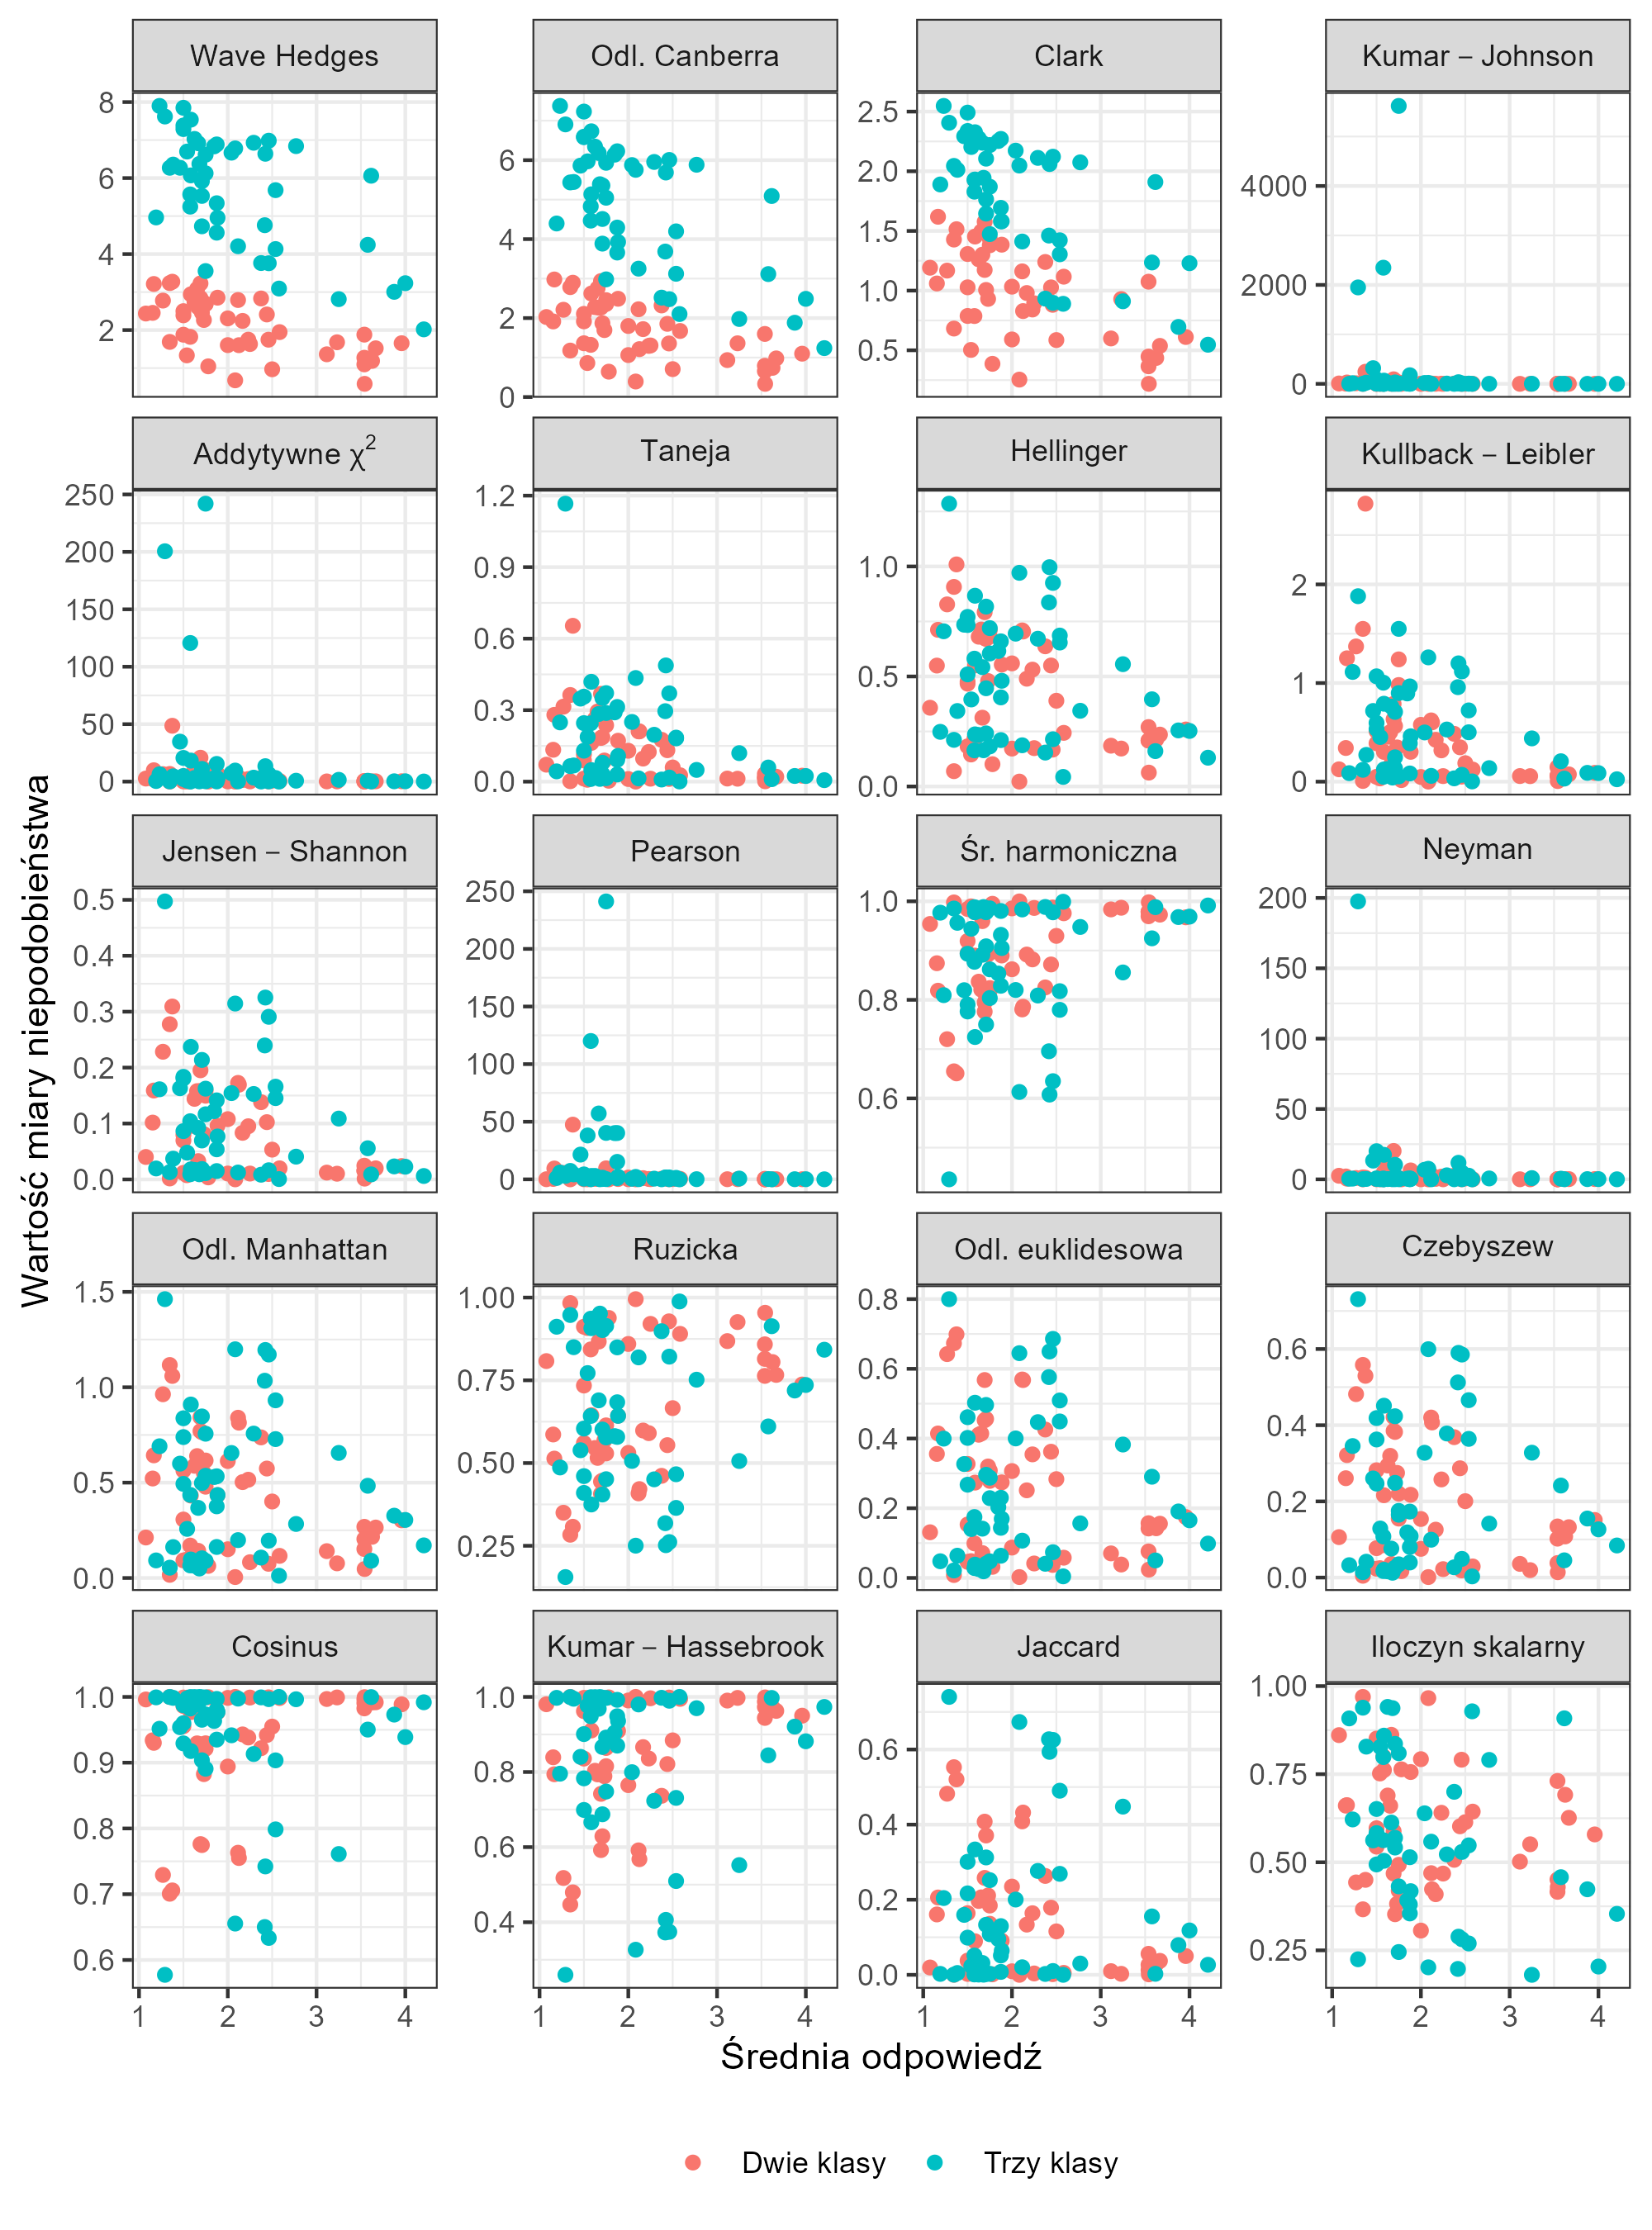
\includegraphics[width=5.72917in,height=7.72917in]{figures/avg_vs_measures.png}

}

\caption{\label{fig-avg_vs_measures}Relacje między średnią odpowiedzią a
miarami niepodobieństwa dla dwóch i trzech klas. Miary uporządkowane
według wartości współczynnika determinacji dla dwóch klas}

\end{figure}

Rycina \ref{fig-avg_vs_measures} przedstawia relacje między średnią
odpowiedzią a miarami niepodobieństwa dla dwóch i trzech klas.
Analizując wykresy można zauważyć, że w przypadku części miar zakres
wartości w którym mieszczą się ich wyniki zależny jest od liczby klas
obecnych na rastrach. Do tej grupy należą miary Wave Hedgesa, Canberra
oraz Clarka, natomiast zakres wartości pozostałych miar nie jest zależny
od liczby klas.

Dla miar Kumara-Johnsona, Pearsona, Neymana oraz Addytywnego \(\chi^2\)
widoczne są także pojedyncze punkty znacznie przewyższające wszystkie
pozostałe uzyskaną wartością niepodobieństwa. Wyniki tak znacznie
odstające mają duży wpływ na ostateczny wynik współczynnika determinacji
tych miar. Dla wszystkich czterech miar odstające punkty odpowiadają
grupie tych samych trzech pytań dotyczących wyłącznie par rastrów z
trzema klasami. Pary rastrów związane z odstającymi wynikami
współczynnika determinacji przedstawia Rycina
\ref{fig-pyt_odstajace_kopia}.

\textbf{\emph{Dla każdej ze wspomnianych wcześniej miar, dwa najbardziej
odstające wyniki odpowiadają pytaniom, które należały do podgrupy pytań
o identycznej kompozycji i różnej konfiguracji przestrzennej. Rastry
uwzględnione w tych pytaniach zostały oznaczone na Rycinie
\ref{fig-pyt_odstajace_kopia} jako ``Pytanie A'' oraz ``Pytanie B''.
Różnica we względnej informacji wzajemnej dla tych par rastrów wynosi
0,58 i 0,63. Oznacza to, że rastry różnią się pod względem konfiguracji
w dużym stopniu.}}

\textbf{\emph{Jeden z odstających wyników, oznaczony na Rycinie
\ref{fig-pyt_odstajace_kopia} jako ``Pytanie C'', dotyczy pytania z
podgrupy o różnej kompozycji i konfiguracji. Dla tej pary rastrów
różnica entropii wynosi 1,42, natomiast różnica względnej informacji
wzajemnej wynosi 0,22. Oznacza to, że rastry są bardzo mocno
zróżnicowane pod względem kompozycji, natomiast w małym stopniu różnią
się konfiguracją przestrzenną.}}

\begin{figure}[t]

{\centering 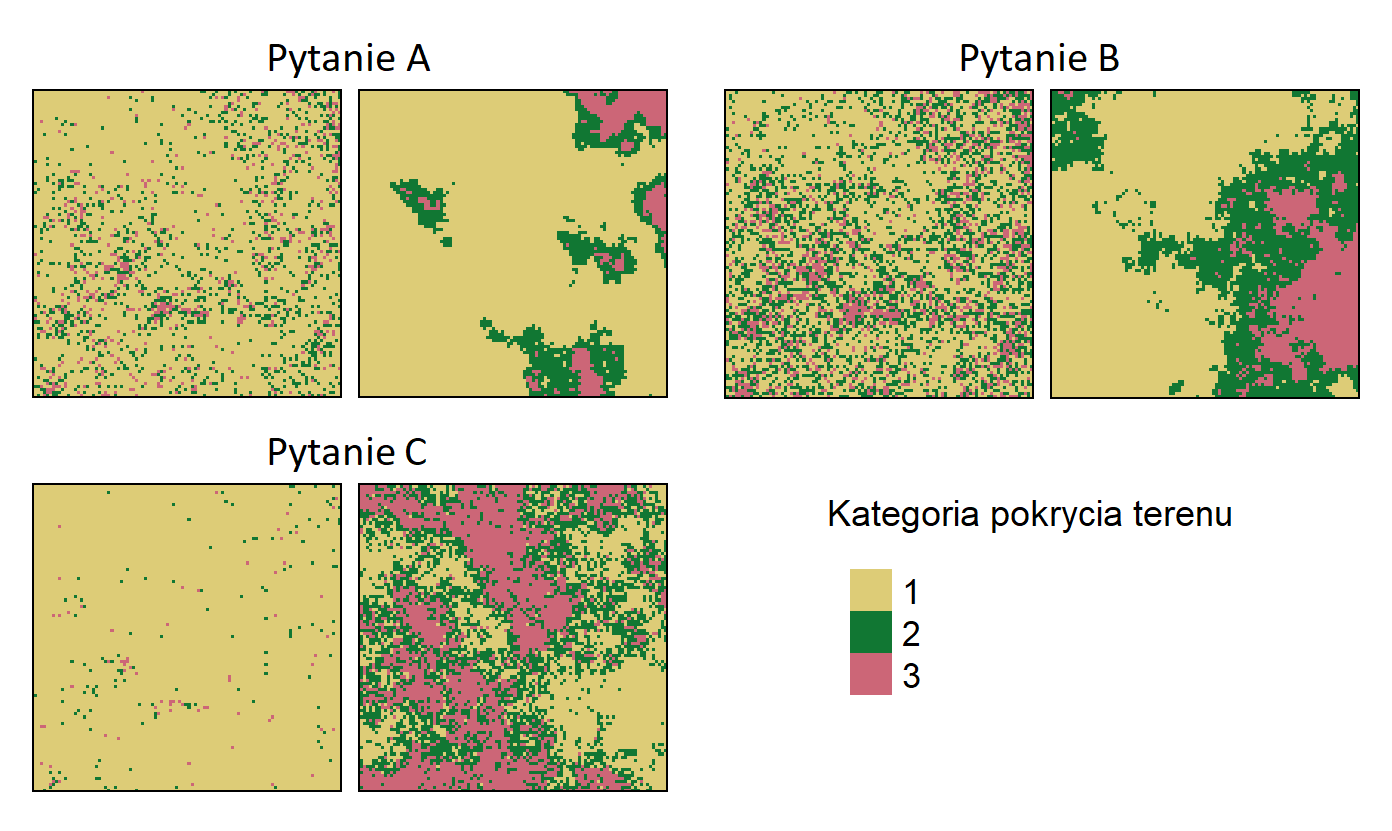
\includegraphics[width=5.10417in,height=3.04167in]{figures/pyt_odstajace_kopia.png}

}

\caption{\label{fig-pyt_odstajace_kopia}Pytania związane z odstającymi
wynikami współczynnika determinacji w relacji ze średnią odpowiedzi}

\end{figure}

\hypertarget{odpowiedzi-a-ruxf3ux17cnice-miux119dzy-miarami-z-teorii-informacji}{%
\section{Odpowiedzi a różnice między miarami z teorii
informacji}\label{odpowiedzi-a-ruxf3ux17cnice-miux119dzy-miarami-z-teorii-informacji}}

Niniejszy podrozdział koncentruje się na badaniu relacji pomiędzy
odpowiedziami ankietowanych a różnicami wartości miar z teorii
informacji. Analiza korelacji przeprowadzona została na podstawie
przygotowanych do ankiety dwóch zbiorów rastrów z dwoma i trzema klasami
oraz dwoma miarami z teorii informacji: entropii oraz względnej
informacji wzajemnej. Te same miary zostały wcześniej wykorzystane w
trakcie przygotowania rastrów do ankiety, w celu potwierdzenia uzyskania
pełnego zakresu kompozycji i konfiguracji przestrzennej (Podrozdział
\ref{sec-symulowanie}). Wyniki korelacji Spearmana sposobów agregacji
odpowiedzi z różnicami entropii i względnej informacji wzajemnej w
podziale na zbiory rastrów z dwoma i trzema klasami przedstawia Tabela
\ref{tbl-mc2_signif_table}.

\hypertarget{tbl-mc2_signif_table}{}
\begin{table}
\caption{\label{tbl-mc2_signif_table}Zestawienie wskaźników korelacji Spearmana sposobów agregacji odpowiedzi
z różnicami entropii i względnej informacji wzajemnej }\tabularnewline

\centering
\begin{tabular}{lllll}
\toprule
\multicolumn{1}{c}{ } & \multicolumn{2}{c}{Dwie klasy} & \multicolumn{2}{c}{Trzy klasy} \\
\cmidrule(l{3pt}r{3pt}){2-3} \cmidrule(l{3pt}r{3pt}){4-5}
Nazwa miary & Różnica entropii & Różnica RMI & Różnica entropii & Różnica RMI\\
\midrule
Średnia odp. & -0.42** & -0.37** & -0.07 & -0.69\\
Mediana odp. & -0.31* & -0.42* & 0.01 & -0.7\\
Moda odp. & -0.21 & -0.43 & 0 & -0.66\\
SD odp. & -0.7*** & 0.24*** & -0.14 & 0.07\\
Różnica entropii & 1*** & -0.29*** & 1*** & -0.43***\\
\addlinespace
Różnica RMI & -0.29* & 1* & -0.43** & 1**\\
\bottomrule
\multicolumn{5}{l}{\rule{0pt}{1em}RMI - względna informacja wzajemna}\\
\multicolumn{5}{l}{\rule{0pt}{1em}Przedziały istotności statystycznej:  0 ‘***’ 0.001 ‘**’ 0.01 ‘*’ 0.05 ‘.’ 0.1 ‘ ’ 1}\\
\end{tabular}
\end{table}

W przypadku dwóch klas, średnia odpowiedź jest negatywnie skorelowana
zarówno z różnicą entropii jak i różnicą względnej informacji wzajemnej.
Inaczej mówiąc, im mniejsza jest różnica entropii lub względnej
informacji wzajemnej pomiędzy parą rastrów, tym wyższa jest wartość
średniej odpowiedzi. Oznacza to, że im mniejsza różnica pomiędzy
właściwościami informacyjnymi pary rastrów, tym według respondentów są
one do siebie bardziej podobne, co potwierdza Rycina
\ref{fig-answer_mean_vs_ent_diff}.

\begin{figure}[t]

{\centering 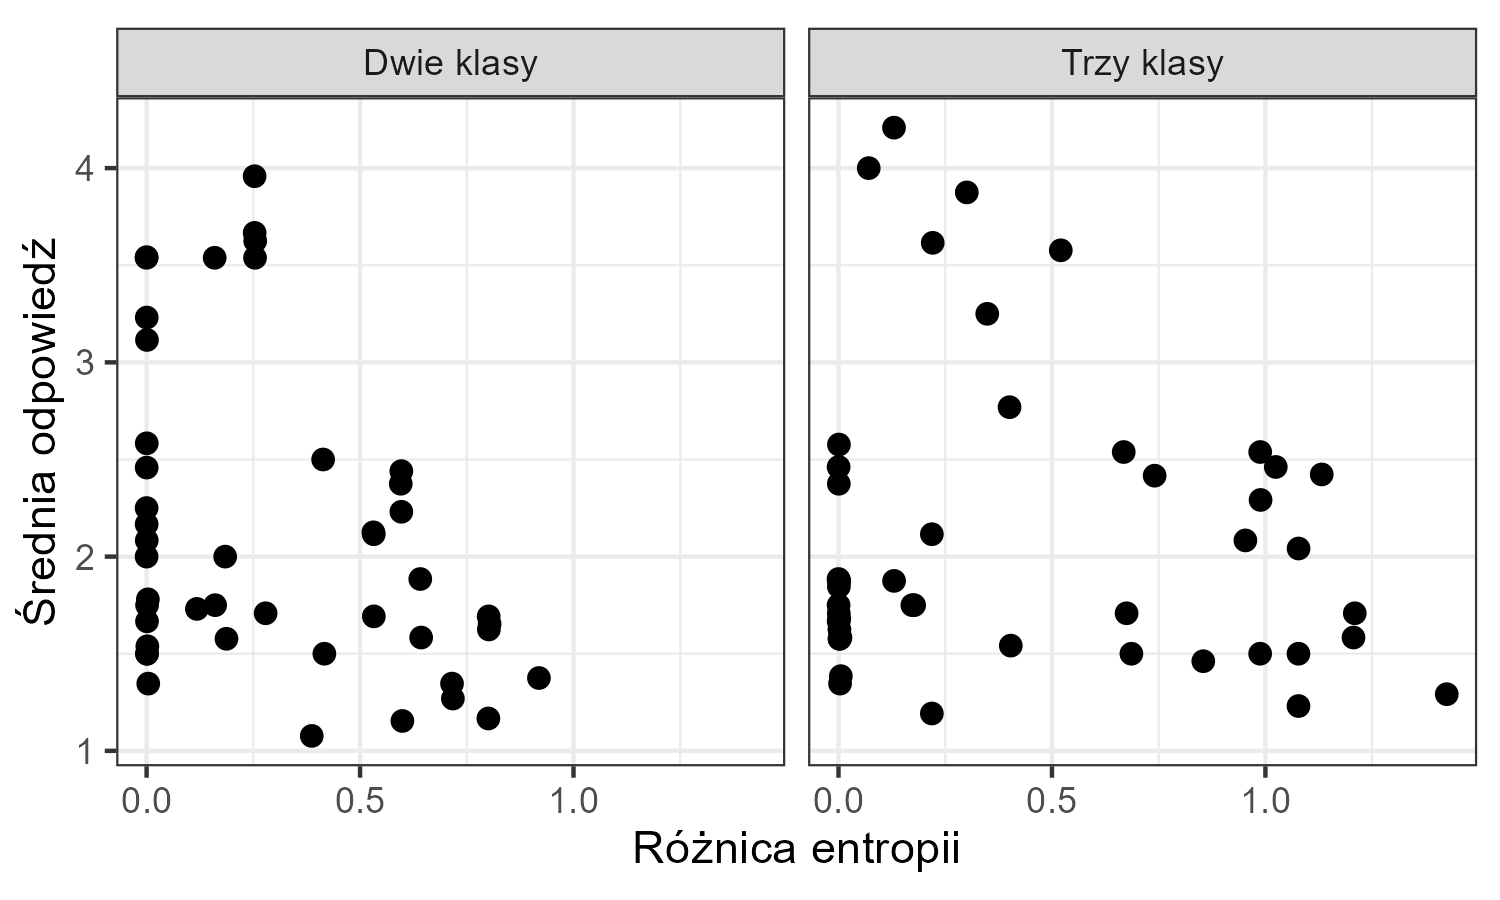
\includegraphics[width=5.20833in,height=3.125in]{figures/answer_mean_vs_ent_diff.png}

}

\caption{\label{fig-answer_mean_vs_ent_diff}Relacja między średnią
odpowiedzią a różnicą entropii dla dwóch i trzech klas}

\end{figure}

W przypadku rastrów z trzema klasami, analiza korelacji Spearmana nie
wykazała istotnej relacji między średnią odpowiedzią a entropią.
Wykazała natomiast negatywną relację z względną informacją wzajemną na
poziomie -0,69, choć istotność statystyczna tej relacji jest bardzo
niska. Niemniej jednak, na Rycinie
\ref{fig-answer_mean_vs_relmutinf_diff} można zauważyć, że dla różnic
względnej informacji wzajemnej z zakresu od 0 do 0,25, średnia odpowiedź
gwałtownie maleje. Wskazuje to na występowanie potencjalnej, nieliniowej
relacji między tymi zmiennymi, co sugeruje potrzebę dalszych badań w
celu jej potwierdzenia.

\begin{figure}[t]

{\centering 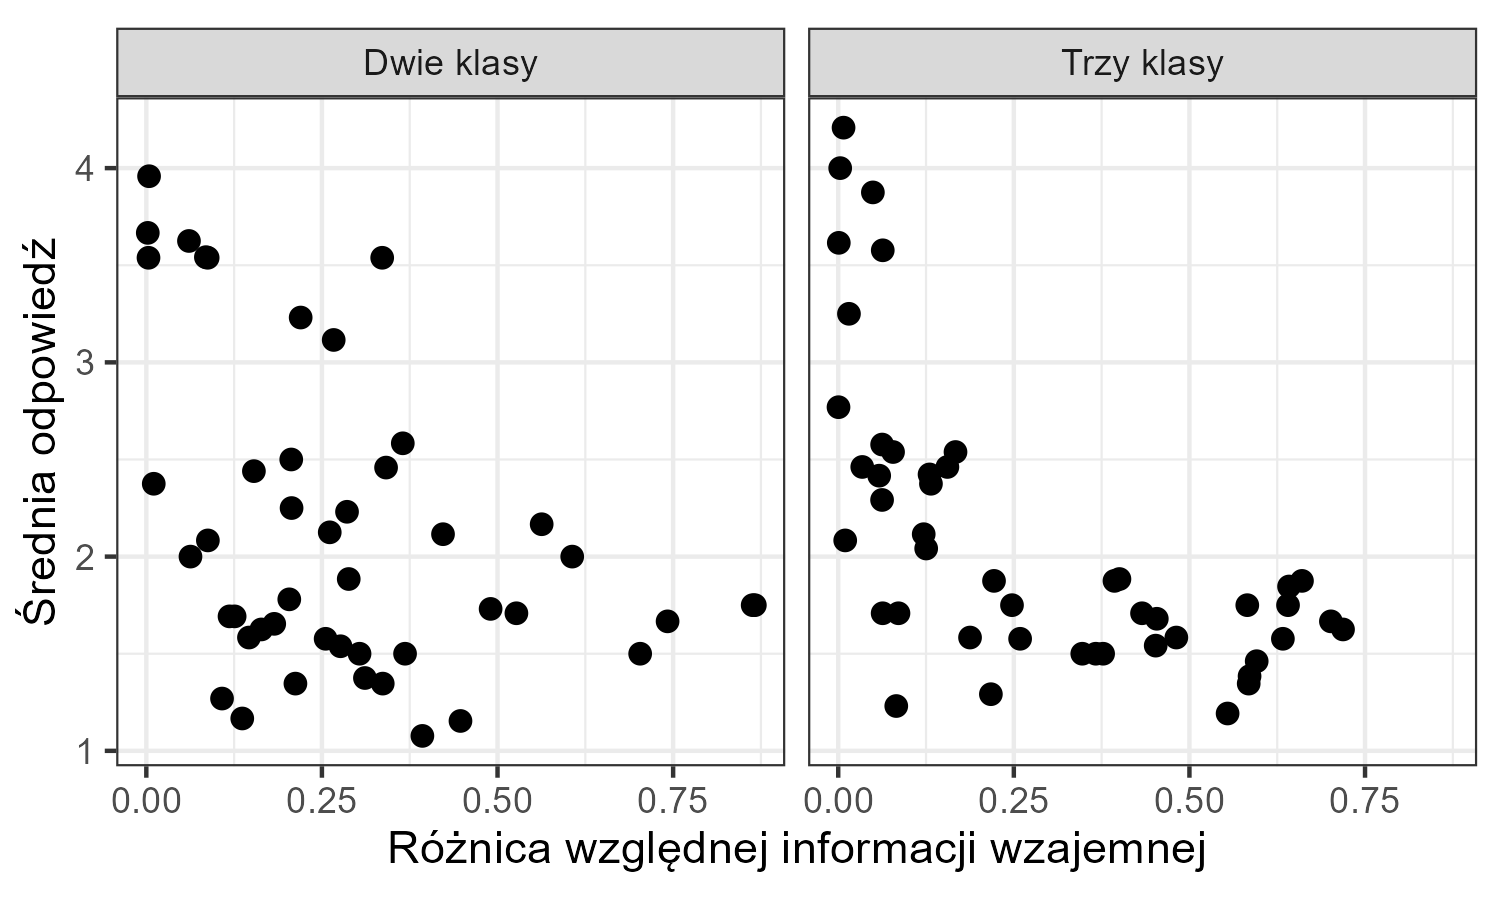
\includegraphics[width=5.20833in,height=3.125in]{figures/answer_mean_vs_relmutinf_diff.png}

}

\caption{\label{fig-answer_mean_vs_relmutinf_diff}Relacja między średnią
odpowiedzią a różnicą względnej informacji wzajemnej dla dwóch i trzech
klas}

\end{figure}

Odchylenie standardowe odpowiedzi dla dwóch klas jest wyraźnie
negatywnie skorelowane z różnicą entropii. Im większa była różnica w
entropii między parą rastrów, tym mniejsze było zróżnicowanie
odpowiedzi. Oznacza to, że respondenci są tym bardziej ze sobą zgodni,
im bardziej rastry różnią się od siebie pod względem entropii. Natomiast
wynik wskaźnika korelacji odchylenia standardowego ze względną
informacją wzajemną nie jest istotny statystycznie.

Odchylenie standardowe odpowiedzi dla trzech klas nie wykazuje istotnej
statystycznie relacji z różnicami między miarami z teorii informacji.

\bookmarksetup{startatroot}

\hypertarget{analiza-zruxf3ux17cnicowania-wybranych-miar-niepodobieux144stwa-na-podstawie-danych-corine-land-cover}{%
\chapter{Analiza zróżnicowania wybranych miar niepodobieństwa na
podstawie danych CORINE Land
Cover}\label{analiza-zruxf3ux17cnicowania-wybranych-miar-niepodobieux144stwa-na-podstawie-danych-corine-land-cover}}

W tym rozdziale skupiono się na próbie wyjaśnienia różnic między
wynikami czterech wybranych miar niepodobieństwa: odległości
euklidesowej, miary Jensena-Shannona, Wave Hedgesa oraz Tanejy, które
zostały obliczone dla obszarów wydzielonych z danych rastrowych o
pokryciu terenu CORINE Land Cover. W pierwszej sekcji omówione jest
zastosowane podejście do porównania tych miar oraz wykorzystane w tym
celu dane przestrzenne CORINE Land Cover. Następnie, w drugiej sekcji
opisano relacje między poszczególnymi miarami niepodobieństwa.
Przedstawiony jest także sposób wyboru obszarów, dla których miary
niepodobieństwa wykazały największe zróżnicowanie a także opis tych
obszarów. W ostatniej sekcji tego rozdziału opisana jest relacja
czterech miar niepodobieństwa ze zmianami kompozycji i konfiguracji
przestrzennej.

\hypertarget{poruxf3wnanie-wybranych-miar-niepodobieux144stwa-w-kontekux15bcie-okreux15blania-zmian-kategorii-pokrycia-terenu}{%
\section{Porównanie wybranych miar niepodobieństwa w kontekście
określania zmian kategorii pokrycia
terenu}\label{poruxf3wnanie-wybranych-miar-niepodobieux144stwa-w-kontekux15bcie-okreux15blania-zmian-kategorii-pokrycia-terenu}}

Dalsza część porównania miar niepodobieństwa opierała się na analizie
wyników wybranych miar przy zastosowaniu w analizie zmian pokrycia
terenu na podstawie danych rzeczywistych. W tym celu zostały
wykorzystane dane CORINE Land Cover dla obszaru Polski dla lat 1990 i
2018, które zostały opisane w Podrozdziale \ref{sec-CLC}. Dla
uproszczenia analizy, dane CLC zostały zreklasyfikowane tak aby
uwzględniały wyłącznie dwie kategorie pokrycia terenu: lasy i pozostałe
obszary.

Do oceny zmian pokrycia terenu zastosowano metody oparte na analizie
struktur przestrzennych, opisane dokładniej w Podrozdziale
\ref{sec-pattern-based}. Dane wejściowe zostały podzielone na regularną
siatkę kwadratów o wymiarach 100 na 100 komórek rastra (10 na 10 km). W
ten sposób, obszar badań podzielony został na 3337 mniejszych jednostek.
Następnie, dla tych obszarów obliczone zostały zmiany ich struktur
przestrzennych dla danych z 1990 i 2018 roku wykorzystując do tego
cztery miary niepodobieństwa wybrane na podstawie różnych kryteriów:

\begin{itemize}
\tightlist
\item
  Odległość euklidesowa -- najpopularniejsza miara niepodobieństwa,
  która nie jest zależna od liczby klas
\item
  Jensen-Shannon -- miara niepodobieństwa, która również nie jest
  zależna od liczby klas a jest wykorzystywana w pracach dotyczących
  podobieństwa struktur przestrzennych \textbf{\emph{(REF)}}
\item
  Wave Hedges -- miara niepodobieństwa, która jest zależna od liczby
  klas, ale która dała najwyższą wartość współczynnika determinacji dla
  średniej odpowiedzi dla dwóch klas oraz jedną z najwyższych dla trzech
  klas
\item
  Taneja -- miara niepodobieństwa, która nie jest zależna od liczby
  klas, ale która dała relatywnie wysokie wartości współczynnika
  determinacji dla odchylenia standardowego odpowiedzi dla dwóch oraz
  trzech klas
\end{itemize}

Ze względu na to że oryginalnie wyniki tych miar mieszczą się w różnych
przedziałach wartości, zostały one przeskalowane do zakresu od 0 do 100.
Dzięki temu można łatwiej ze sobą porównać wyniki tych miar. Należy
jednak wziąć pod uwagę, że w takiej sytuacji wartość miar równa 0
niekoniecznie będzie oznaczać całkowity brak zmian w strukturze
przestrzennej, a po prostu najmniejszą zmianę z całego zbioru danych.
Wartość 100 natomiast reprezentować będzie obszary o największej zmianie
struktury przestrzennej.

\begin{figure}[t]

{\centering 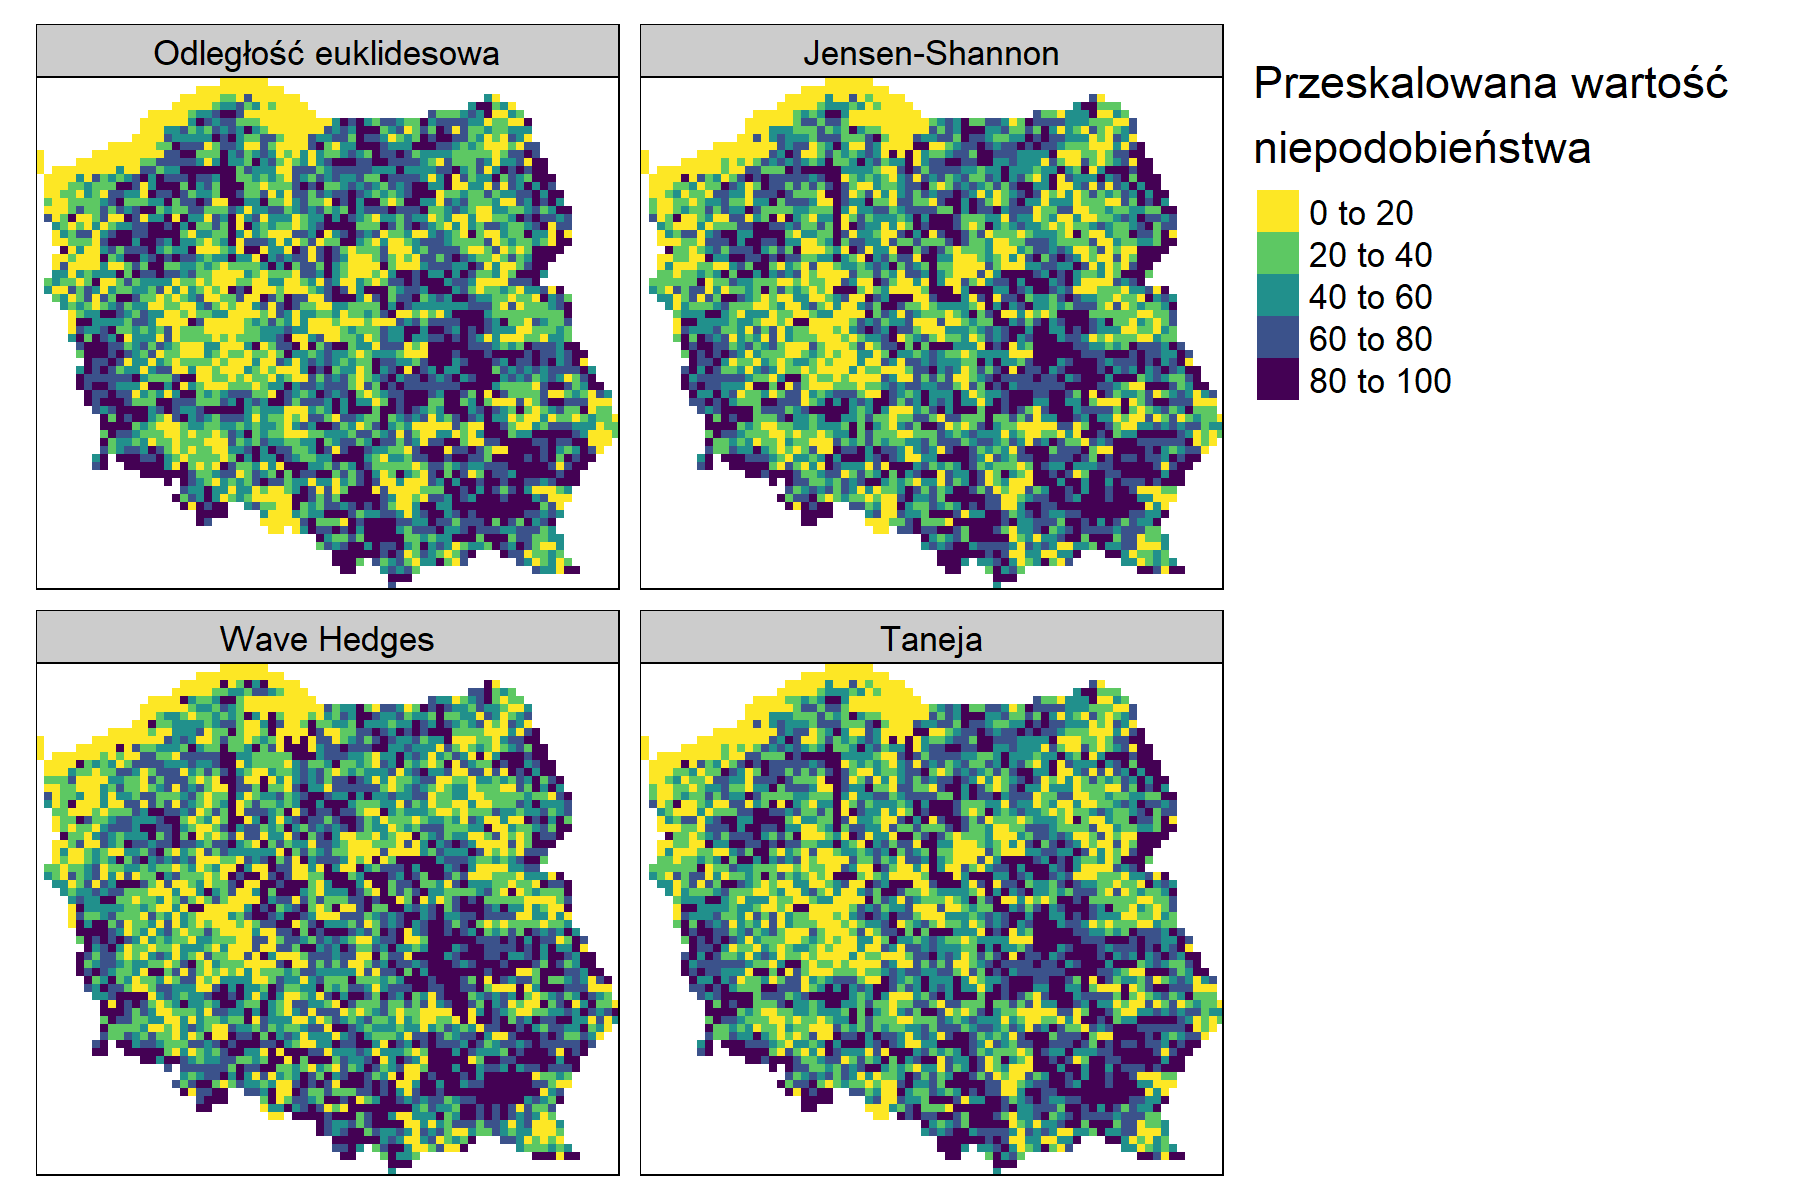
\includegraphics[width=5.20833in,height=3.46875in]{figures/zestawienie_miar1.png}

}

\caption{\label{fig-zestawienie_miar1}Zestawienie wyników czterech miar
niepodobieństwa}

\end{figure}

Uwzględnione miary niepodobieństwa wykazują między sobą na tyle silne
relacje, że na pierwszy rzut oka trudno zauważyć istotne różnice
pomiędzy nimi na mapach (Rycina \ref{fig-zestawienie_miar1}). Dlatego
też, aby dokładniej zrozumieć różnice w wynikach tych miar, konieczna
jest głębsza analiza danych uwzględniająca bezpośrednie porównanie ze
sobą wyników miar dla obszarów o największych różnicach wartości.

\hypertarget{poruxf3wanie-wynikuxf3w-miar-niepodobieux144stwa}{%
\section{Porówanie wyników miar
niepodobieństwa}\label{poruxf3wanie-wynikuxf3w-miar-niepodobieux144stwa}}

W celu wskazania obszarów dla których miary niepodobieństwa dają
najbardziej zróżnicowane wyniki, dla każdego obszaru obliczone zostało
odchylenie standardowe czterech wybranych miar niepodobieństwa.
Następnie wybrano obszary, dla których odchylenie standardowe miar
znalazło się w 1\% najwyższych wyników. Pozwoliło to na wskazanie 12
obszarów, dla których wyniki miar niepodobieństwa są najbardziej
zróżnicowane z całego zbioru danych. Próg dla najwyższych 1\% odchyleń
standardowych wyniósł 31,03. Wyniki powyżej tego progu wskazują na
bardzo duże zróżnicowanie wyników miar niepodobieństwa. Dodatkowo,
wybrano cztery obszary dla których wartości miar Tanejy i
Jensena-Shannona różniły się od siebie w znacznym stopniu.

\begin{figure}[t]

{\centering 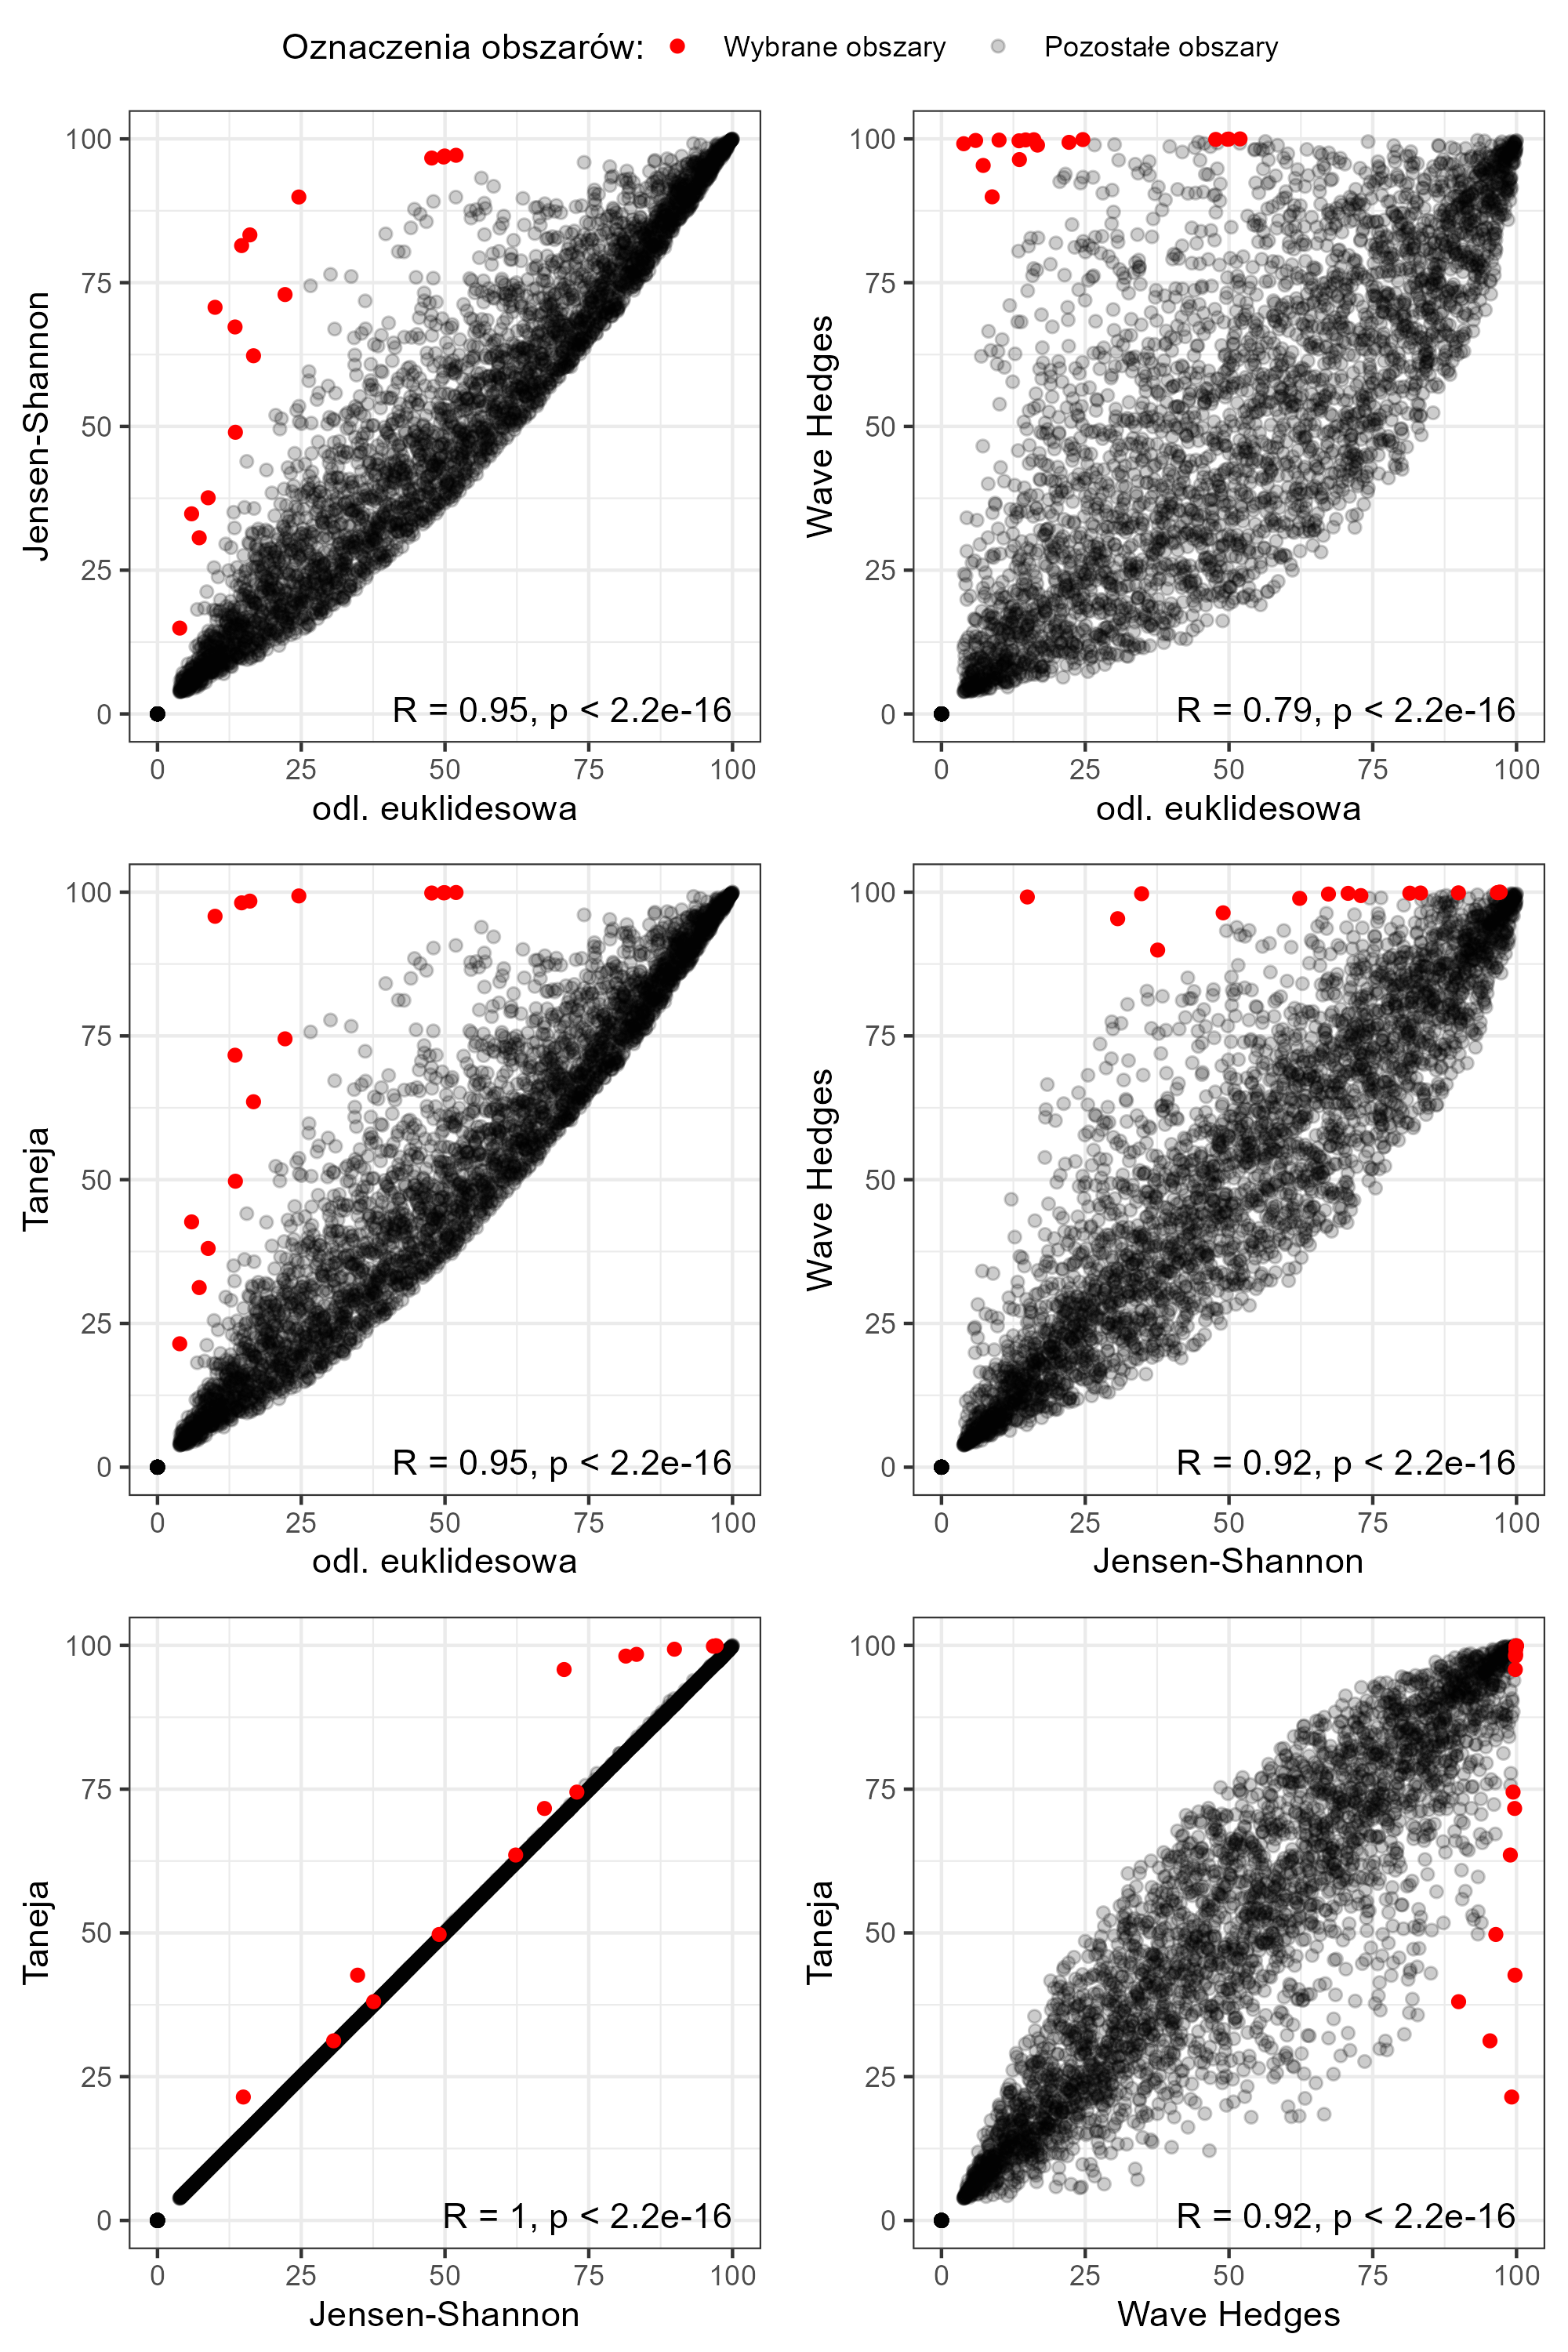
\includegraphics[width=5.20833in,height=7.8125in]{figures/relacje_miar1.png}

}

\caption{\label{fig-relacje_miar1}Relacje między czterema wybranymi
miarami niepodobieństwawa}

\end{figure}

Na podstawie wykresów na Rycinie \ref{fig-relacje_miar1} możemy
zauważyć, że wszystkie cztery miary niepodobieństwa są ze sobą silnie
skorelowane. W szczególności miary Jensena-Shannona oraz Tanejy
charakteryzują się prawie pełną zgodnością. Wyjątek stanowią obszary
oznaczone kolorem czerwonym, które reprezentują sytuacje o dużym
zróżnicowaniu wyników miar niepodobieństwa. Obszary te widocznie odstają
także w przypadku pozostałych relacji miar. Najsłabszą relację wykazują
miara Wave Hedgesa z odległością euklidesową.

\begin{figure}[t]

{\centering 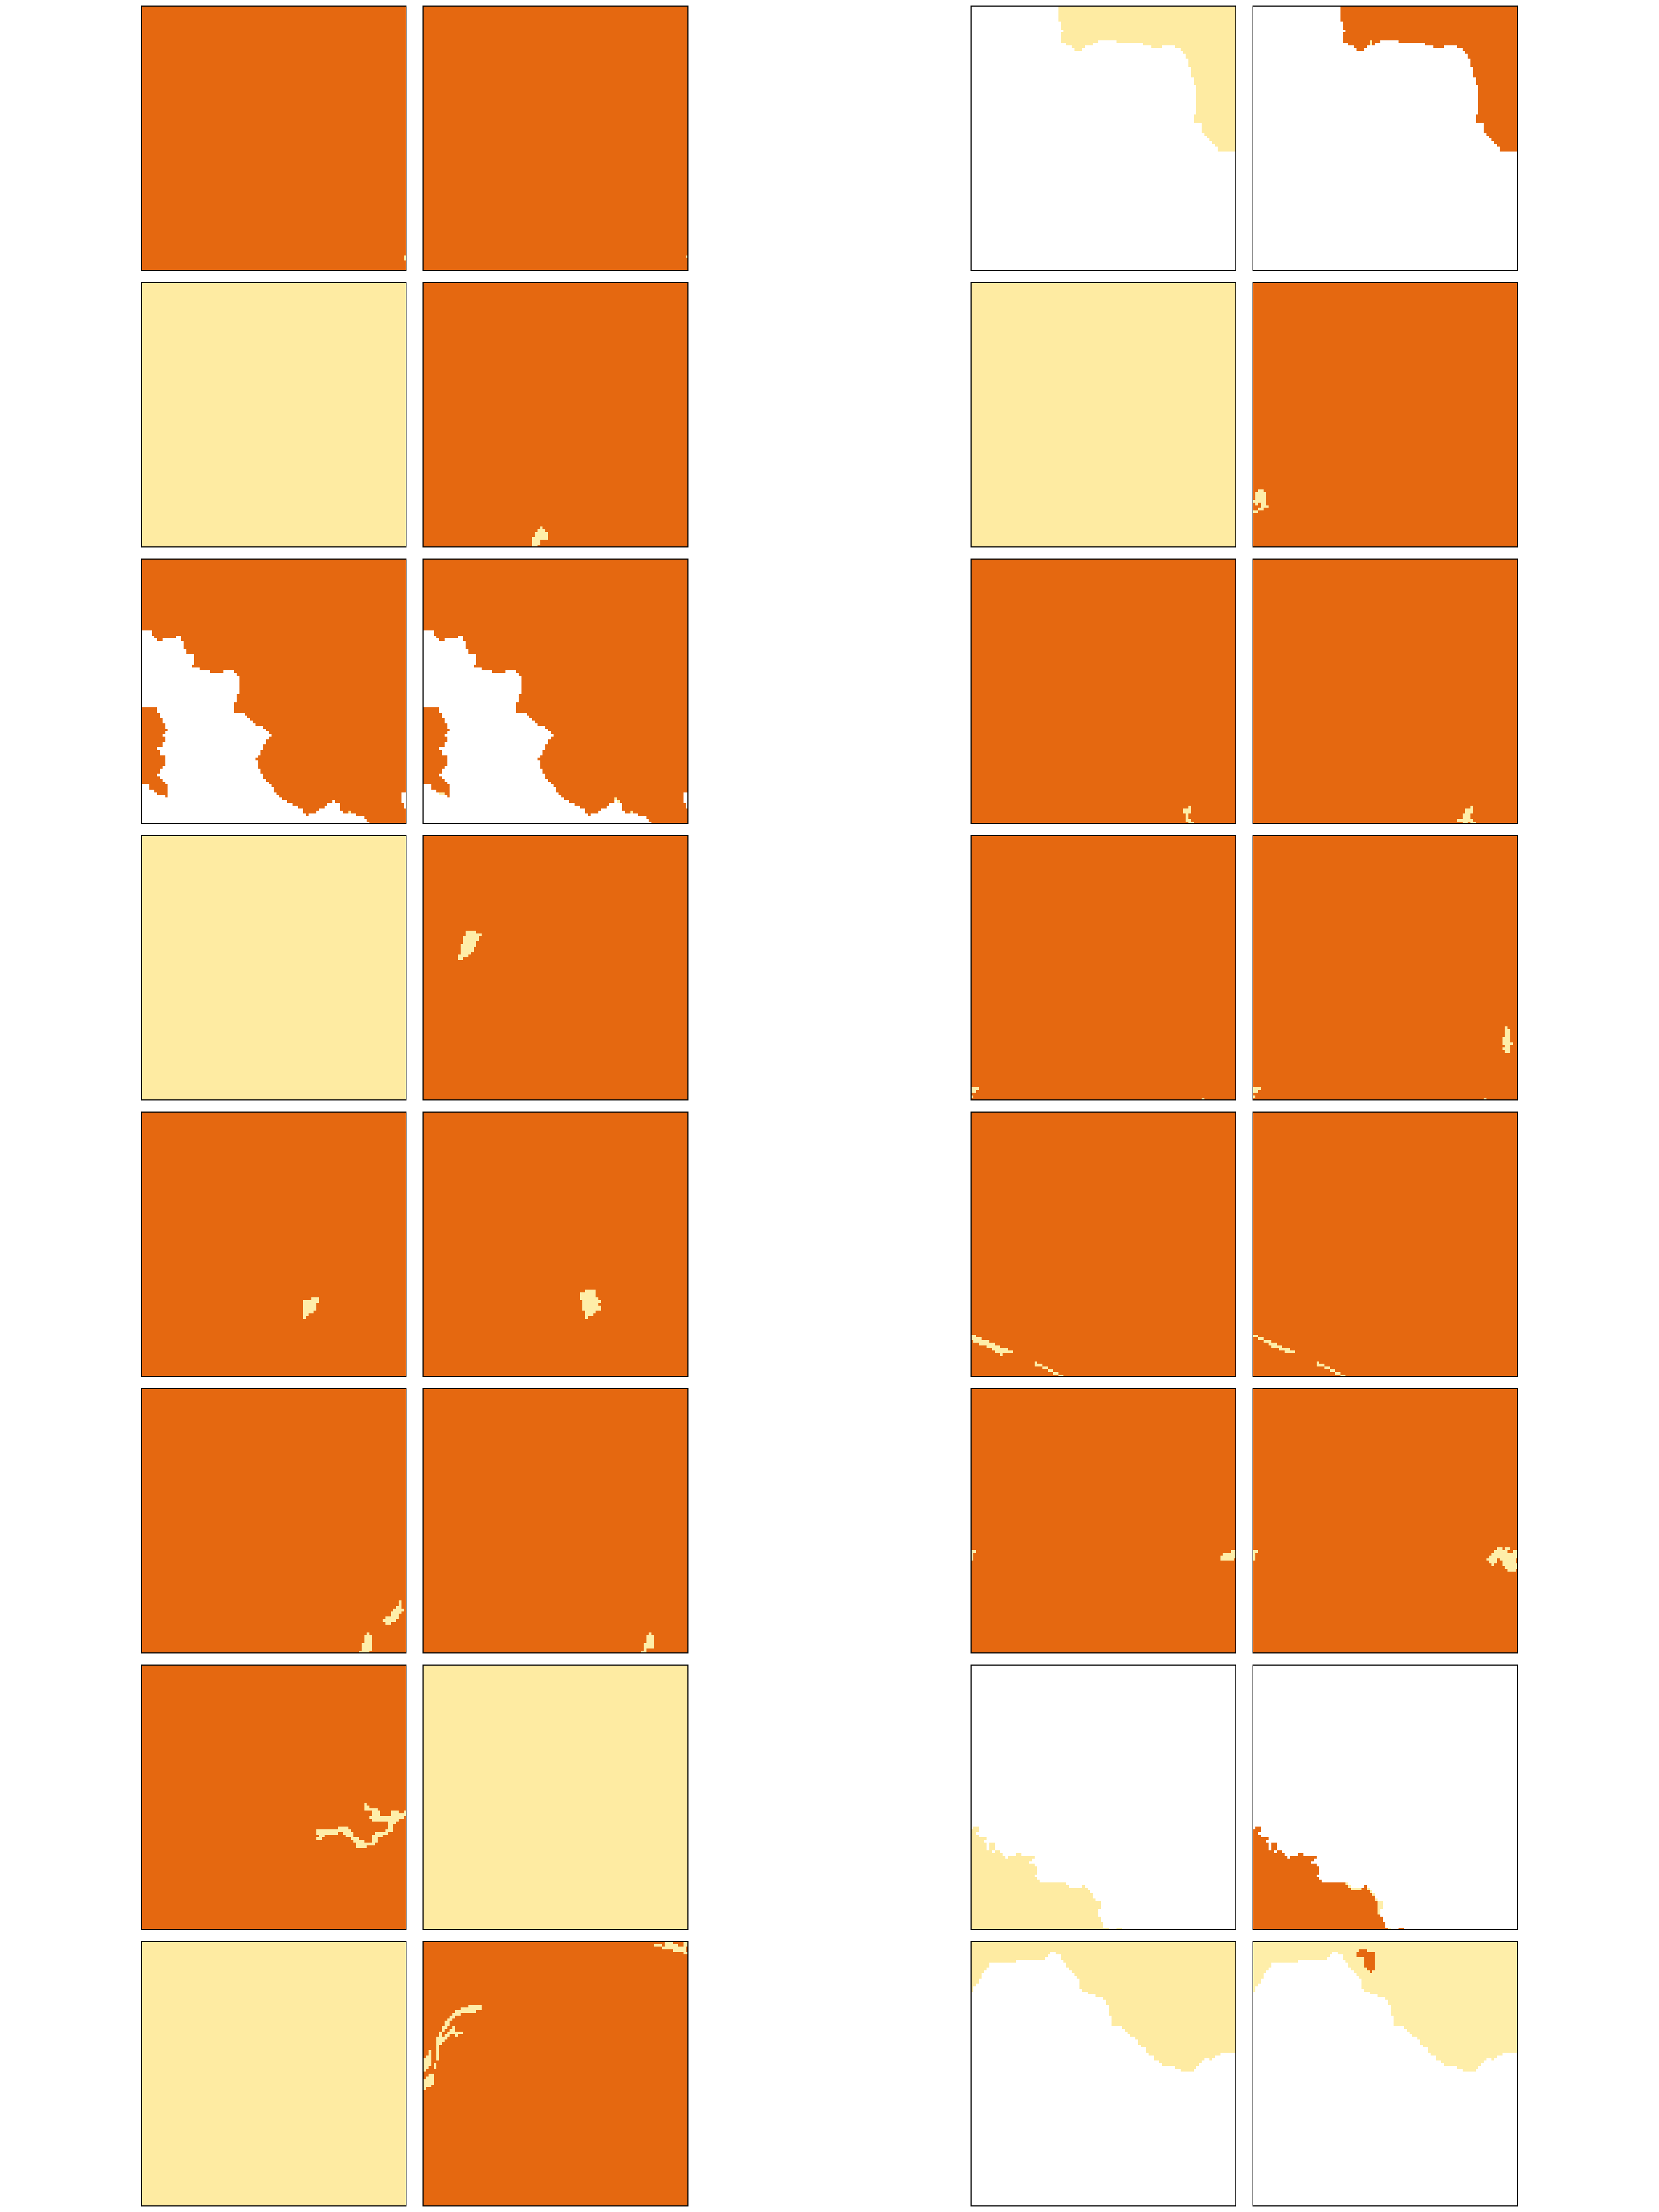
\includegraphics[width=5.20833in,height=6.9375in]{figures/obszary_odst.png}

}

\caption{\label{fig-obszary_odst}Obszary dla których miary
niepodobieństwa dają najbardziej zróżnicowane wyniki. Posortowane
malejąco według odchylenia standardowego miar}

\end{figure}

\hypertarget{tbl-obszary_odst_tabela}{}
\begin{table}
\caption{\label{tbl-obszary_odst_tabela}Zestawienie wyników czterech miar niepodobieństwa obszarów odstających.
Posortowane malejąco według odchylenia standardowego miar }\tabularnewline

\centering
\begin{tabular}{>{\raggedleft\arraybackslash}p{1.5cm}>{\raggedleft\arraybackslash}p{1.5cm}>{\raggedleft\arraybackslash}p{1.5cm}>{\raggedleft\arraybackslash}p{2.2cm}>{\raggedleft\arraybackslash}p{1.8cm}>{\raggedleft\arraybackslash}p{1.5cm}>{\raggedleft\arraybackslash}p{1.5cm}}
\toprule
Numer obszaru & Różnica entropii & Różnica RMI & odległość euklidesowa & Jensen-Shannon & Wave Hedges & Taneja\\
\midrule
1 & 0.001 & 0.241 & 3.87 & 14.93 & 99.16 & 21.46\\
2 & 0.013 & 0.822 & 10.01 & 70.71 & 99.79 & 95.80\\
3 & 0.028 & 0.365 & 14.63 & 81.44 & 99.82 & 98.14\\
4 & 0.028 & 0.460 & 16.07 & 83.30 & 99.85 & 98.44\\
5 & 0.004 & 0.088 & 5.94 & 34.80 & 99.73 & 42.66\\
\addlinespace
6 & 0.009 & 0.119 & 7.25 & 30.64 & 95.38 & 31.24\\
7 & 0.048 & 0.317 & 24.58 & 89.90 & 99.88 & 99.34\\
8 & 0.022 & 0.184 & 13.49 & 67.30 & 99.67 & 71.64\\
9 & 0.021 & 0.058 & 13.55 & 48.98 & 96.40 & 49.73\\
10 & 0.012 & 0.157 & 8.81 & 37.59 & 89.93 & 38.04\\
\addlinespace
11 & 0.026 & 0.008 & 16.70 & 62.29 & 98.92 & 63.55\\
12 & 0.037 & 0.069 & 22.18 & 72.93 & 99.40 & 74.49\\
13 & 0.097 & 0.475 & 47.69 & 96.67 & 99.91 & 99.85\\
14 & 0.088 & 0.698 & 49.76 & 96.85 & 99.94 & 99.88\\
15 & 0.098 & 0.541 & 49.94 & 97.03 & 99.97 & 99.91\\
\addlinespace
16 & 0.110 & 0.379 & 51.92 & 97.15 & 100.00 & 99.94\\
\bottomrule
\multicolumn{7}{l}{\rule{0pt}{1em}RMI - względna informacja wzajemna}\\
\end{tabular}
\end{table}

Obszary, dla których miary niepodobieństwa wykazały największe
zróżnicowanie, zostały przedstawione na Rycinie \ref{fig-obszary_odst}.
Wśród tych obszarów można wyróżnić dwie główne grupy: pierwsza grupa
obejmuje obszary, na których nastąpiły bardzo niewielkie zmiany,
natomiast druga grupa to obszary, na których doszło do całkowitej lub
prawie całkowitej zmiany kategorii pokrycia terenu. Każda z tych grup
liczy po 8 obszarów.

Warto zauważyć, że miara Wave Hedgesa dla punktów odstających wykazała
wyłącznie bardzo wysokie wartości powyżej 89. Oznacza to, że w bardzo
specyficznych sytuacjach ta miara wskazuje na podobny stopień zmian
pokrycia terenu zarówno w przypadku obszarów o rzeczywiście bardzo
dużych, jak i niewielkich zmianach.

W przypadku każdego z wybranych obszarów, miara Tanejy wskazuje na
większe zmiany pokrycia terenu w porównaniu do miary Jensena-Shannona. W
przypadku tych dwóch miar występują sytuacje, gdzie niektórym obszarom,
na których doszło do prawie całkowitej zmiany pokrycia terenu,
przypisane są bardzo wysokie wartości powyżej 80, podczas gdy innym
obszarom o podobnym stopniu zmian przypisane są wartości nawet poniżej
40. Analogiczna sytuacja występuje także w przypadku obszarów
charakteryzujących się niewielkimi zmianami pokrycia terenu.

\hypertarget{miary-niepodobieux144stwa-a-kompozycja-i-konfiguracja-przestrzenna}{%
\section{Miary niepodobieństwa a kompozycja i konfiguracja
przestrzenna}\label{miary-niepodobieux144stwa-a-kompozycja-i-konfiguracja-przestrzenna}}

\hypertarget{tbl-cztery_miary_ent_relmutinf}{}
\begin{table}
\caption{\label{tbl-cztery_miary_ent_relmutinf}Zestawienie korelacji Spearmana pomiędzy czterema wybranymi miarami
niepodobieństwa a różnicą entropii i różnicą względnej informacji
wzajemnej (RMI) }\tabularnewline

\centering
\begin{tabular}{lrr}
\toprule
Miara niepodobieństwa & Różnica entropii & Różnica RMI\\
\midrule
odległość euklidesowa & 0.71 & 0.42\\
miara Jensena-Shannona & 0.78 & 0.55\\
miara Wave Hedgesa & 0.80 & 0.67\\
miara Tanejy & 0.78 & 0.55\\
\bottomrule
\end{tabular}
\end{table}

W celu oceny stopnia zależności wybranych miar niepodobieństwa od zmian
w kompozycji i przestrzennej konfiguracji obszarów, przeprowadzono
analizę ich korelacji Spearmana z dwiema miarami z teorii informacji:
entropią oraz względną informacją wzajemną. Wyniki te umożliwiają
oszacowanie wpływu zmian w kompozycji i konfiguracji przestrzennej
obszarów na wyniki miar niepodobieństwa. Im wyższa wartość korelacji z
różnicą entropii lub różnicą względnej informacji wzajemnej, tym
teoretycznie większy wpływ mają zmiany kompozycji lub konfiguracji
przestrzennej na wyniki danej miary.

Analiza wyników korelacji przedstawionych w Tabeli
\ref{tbl-cztery_miary_ent_relmutinf} ukazuje, że wszystkie miary
wykazują silną relację z różnicą entropii na zbliżonym poziomie,
wynoszącym między 0,71 a 0,8. Miary wykazują natomiast umiarkowaną
relację z różnicą względnej informacji wzajemnej, których zakres
wartości mieści się w przedziale od 0,42 do 0,67. Najsilniejszy związek
z obiema miarami z teorii informacji wykazuje miara Wave Hedgesa. Miary
Tanejy i Jensena-Shannona uzyskały identyczne wyniki w przypadku obu
miar, natomiast najsłabszą relację w obu przypadkach wykazuje odległość
euklidesowa. Wyniki te oznaczają, że w przypadku tych czterech miar
niepodobieństwa większy wpływ na ostateczny wynik mają zmiany udziałów
kategorii w rastrze niż zmiany sąsiadowania ze sobą kategorii.

\begin{figure}[t]

{\centering 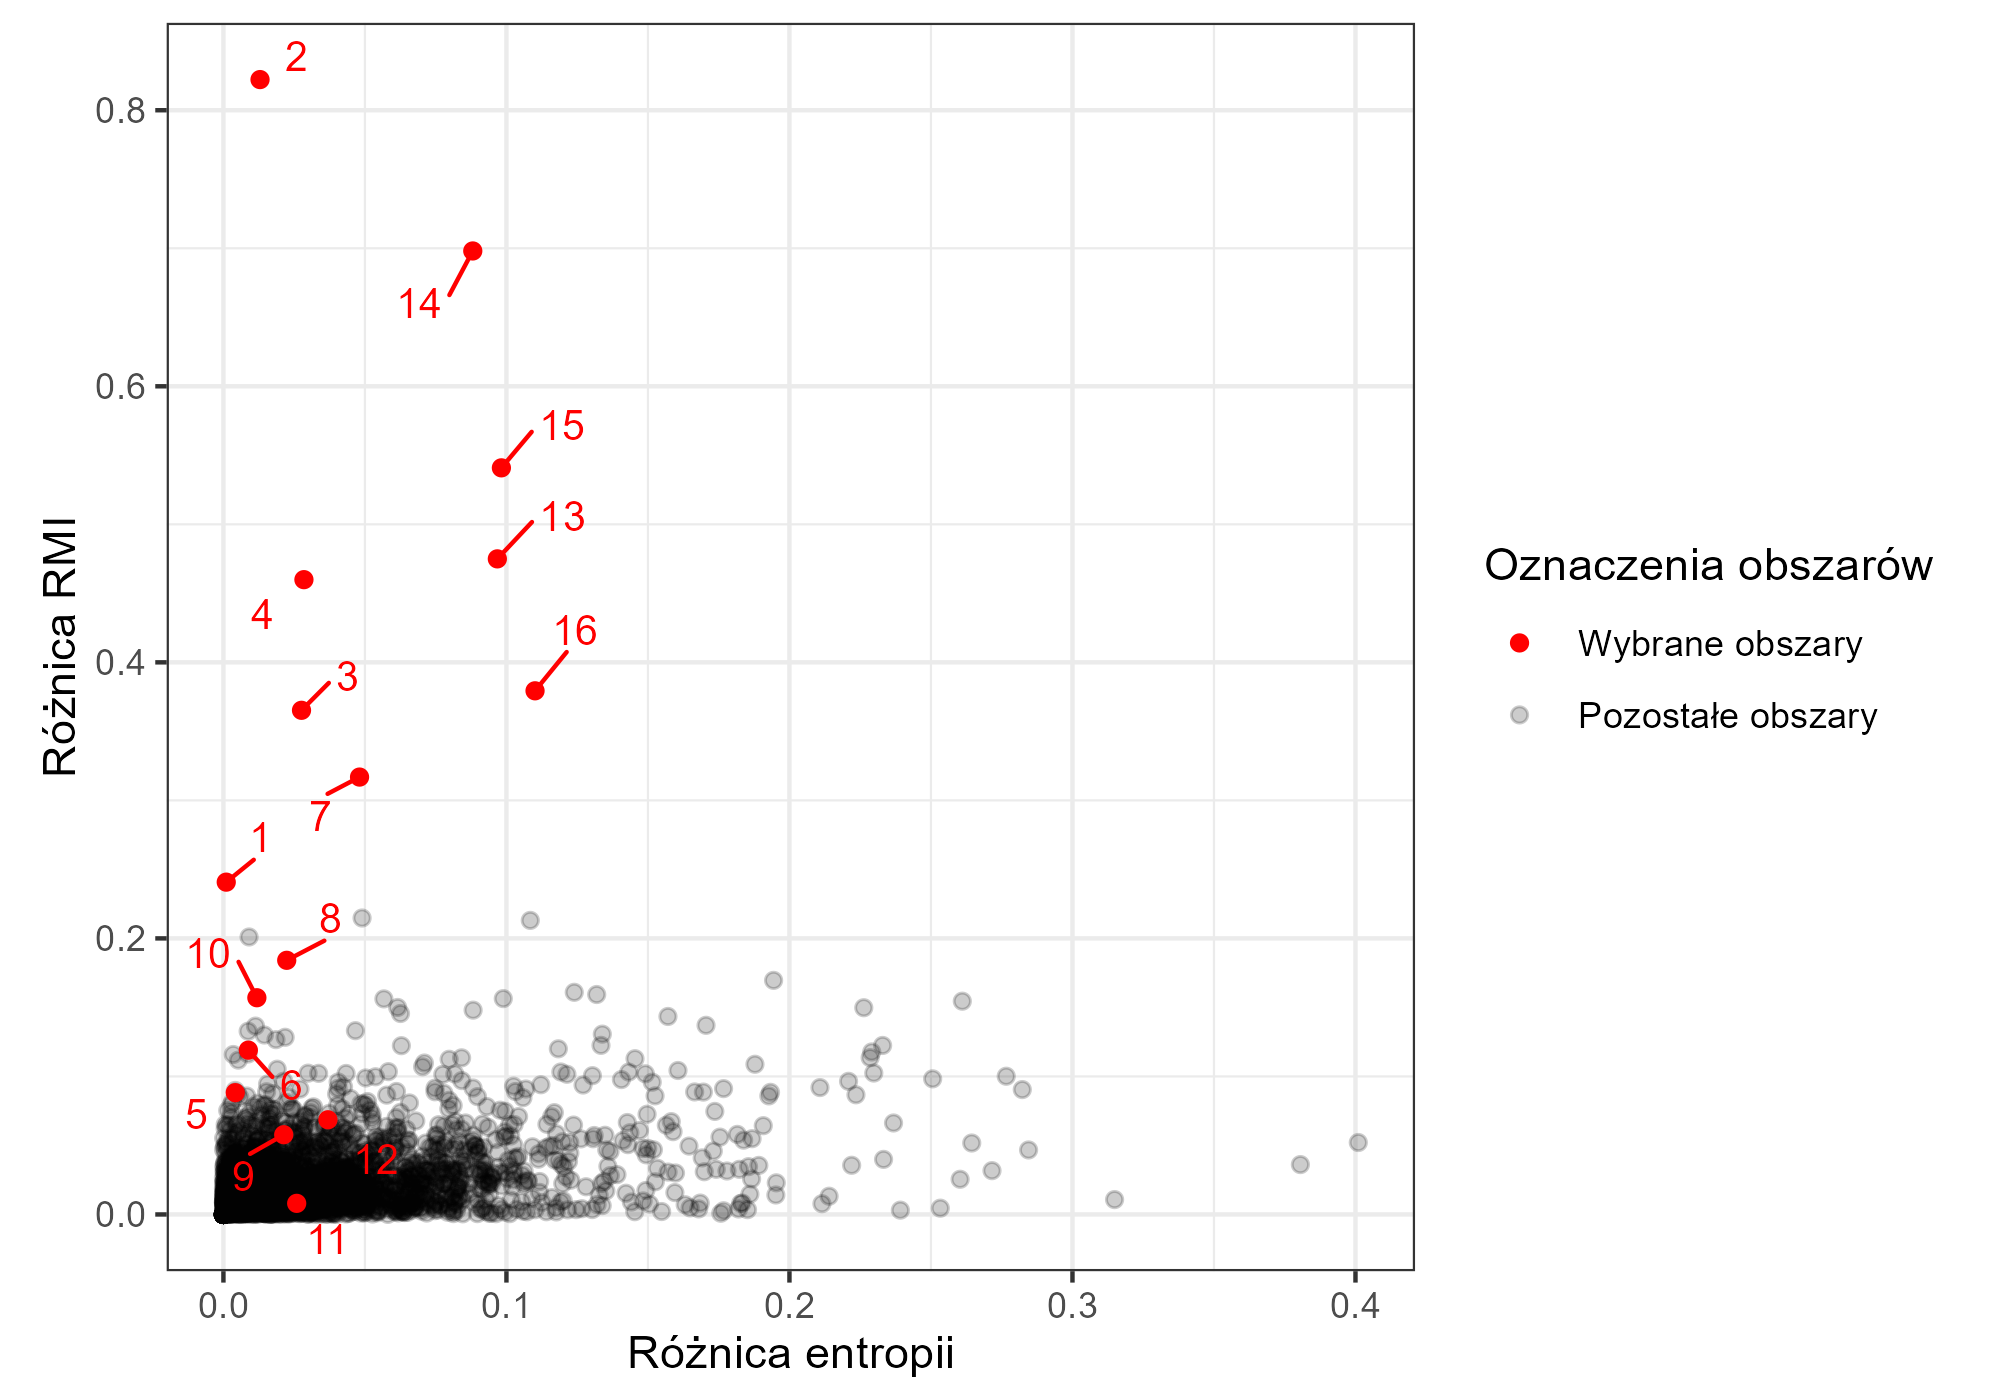
\includegraphics[width=5.20833in,height=3.64583in]{figures/clc_ent_vs_relmutinf.png}

}

\caption{\label{fig-clc_ent_vs_relmutinf}Relacja różnicy entropii z
różnicą względnej informacji wzajemnej (RMI) dla wydzielonych obszarów}

\end{figure}

Na podstawie Ryciny \ref{fig-clc_ent_vs_relmutinf}, która przedstawia
rozkład wartości różnicy entropii i różnicy względnej informacji
wzajemnej, można zauważyć, że dla znacznej części obszarów wartości obu
tych miar znajdują się w przedziale od 0 do 0,1. Oznacza to, że zmiany
kompozycji i przestrzennej konfiguracji na tych obszarach były
stosunkowo niewielkie. Punkty na wykresie oznaczone kolorem czerwonym
reprezentują 16 wcześniej wybranych obszarów charakteryzujących się
wysokim odchyleniu standardowym miar niepodobieństwa. Wartości różnicy
entropii obszarów dla których miary różnią się od siebie najbardziej
mieszczą się w przedziale od 0,02 do 0,11. W przypadku różnic względnej
informacji wzajemnej dla tych obszarów wartości są bardzo zróżnicowane i
mieszczą się w przedziale od 0,008 do ponad 0,82, gdzie 9 z tych
obszarów charakteryzuje się najwyższą różnicą spośród całego zbioru
danych. Analizując rozmieszczenie tych 16 punktów można wywnioskować, że
wyniki miar niepodobieństwa różnią się od siebie znacząco głównie w
przypadku obszarów o niewielkiej różnicy entropii i dosyć dużej różnicy
względnej informacji wzajemnej. To sugeruje, że istotny wpływ na
zgodność wyników miar niepodobieństwa dla różnic między dwoma rastrami
ma to, jak bardzo analizowane rastry różnią się od siebie pod względem
sąsiadowania ze sobą poszczególnych kategorii.

\bookmarksetup{startatroot}

\hypertarget{sec-podsumowanie}{%
\chapter{Podsumowanie}\label{sec-podsumowanie}}

Część miar jest zależna od liczby kategorii. Miary wavehedges, canberra
i clark są zależne, podczas gdy pozostałe nie są. W związku z tym, przy
wykorzystaniu tych miar do analiz pokrycia terenu należy zastanowić się
nad ewentualnym zastosowaniem normalizacji wyników. W tym celu można
zastosować na przykład normalizację min-max. Przykład wpływu tej
procedury na korelacje z wynikami przedstawia rycina XYZ.

\printbibliography[heading=bibintoc, title=Bibliografia]

\end{document}
